\documentclass[11pt, a4paper]{article}
\usepackage[utf8]{inputenc}
\usepackage{mathpazo} % Palatino font
\usepackage{lineno}
\usepackage{setspace}
\usepackage{booktabs}
\usepackage{multirow}
\usepackage{caption}
\captionsetup{labelfont=bf}
\usepackage{graphicx, subfig}
\usepackage{graphicx, subcaption}
\usepackage{float} %so the graphs are not floating around after I put[H]
\usepackage[margin=2cm]{geometry}
\usepackage{indentfirst}
\usepackage{natbib} 
\bibliographystyle{agsm}
\usepackage{amsmath}
\usepackage{tabularx}
\usepackage{hyperref}
\usepackage[dvipsnames]{xcolor}
\hypersetup{
  colorlinks   = true, %Colours links instead of ugly boxes
  urlcolor     = blue, %Colour for external hyperlinks
  linkcolor    = black, %Colour of internal links
  citecolor   = black %Colour of citations
}

\newcommand{\reporttitle}{Changes in microbial community diversity along environmental gradients}
\newcommand{\reportauthor}{Chuxuan Ji}
\newcommand{\supervisor}{Samraat Pawar}
\newcommand{\degreetype}{Master of Research}
\newcommand{\multiref}[2]{\autoref{#1}-\ref{#2}} % from - to

\begin{document}
\begin{spacing}{1.5}
\input{./titlepage.tex}

\section*{Declaration}

I declare that the dissertation is my own work under the supervision of Dr. Samraat Pawar. All sources of information are appropriately referenced. All datasets analysed in this work have been previously published, and data are from the meta-analysis of the Earth Microbiome Project. The work of data sorting, calculation and statistical analysis is done by myself with the suggestion of my supervisor. No portion of the work referred to in the dissertation has been submitted in support of a degree or diploma or other qualification of this or any other university or other institute of learning. 

\clearpage

\section*{Abstract}
\addcontentsline{toc}{section}{Abstract}

Synthesising the vast amounts of data now emerging from field microbial research is a major challenge in ecology. Identifying general patterns in how physical factors, such as temperature, pH or geography (e.g., latitude, altitude) are associated with variation in the composition and diversity of microbial communities has the potential to reveal how they will respond to future environmental changes. Here, I use the  global Environmental Microbiome Project data set to analyze the relationship between bacterial diversity and environmental variables. I use polynomial regression and random forest models to fit the data to explore the environmental variables that had the greatest impact on bacterial diversity at global and local scales. At the global scale, I found that latitude is the most important variable affecting bacterial diversity, which peaks at the subtropics to mid-latitudes. At the local scale, the combination of temperature and pH is the most important variable, with temperature being more important among the two. Overall, random forest captured two times more variation in bacterial diversity than polynomial regression, explaining 40.49\% of the variation in the global data set and 48.06\% in the best-fitted local data set. However, overall, the patterns were weak, because the number of samples across environments is heavily biased, with data from non-saline samples make up more than half of the data set. This may lead to the pattern of non-saline water environment that dominate the entire data set. My research highlights scale-dependence of the link between the environment and bacterial diversity and major gaps in current global data sets. 

\clearpage

\tableofcontents 
\clearpage

\linenumbers
\renewcommand\thesection{\arabic{section}}
\section{Introduction}

Microbes are some of the most abundant and diverse organisms globally, and bacteria are likely to make up the majority of biodiversity and a large proportion (12.73\%) of biomass on Earth \citep{bar2018biomass}. At the same time they play an essential role in building ecosystems and biogeochemical cycles \citep{azam1998microbial}. In the Earth's ecosystems, bacteria regulate many ecosystem processes that are closely linked to climate through complex interactions and feedback mechanisms \citep{azam2007microbial, falkowski2008microbial} while playing a significant role in the carbon \citep{singh2010microorganisms} and nitrogen cycles \citep{kuypers2018microbial}. For instance, microbial respiration accounts for 50$\%$ of global respiration (about 60 billion tonnes of carbon released annually) \citep{hutchins2019climate}, and the world's terrestrial organisms emit about 119 billion tons of carbon annually, half of which comes from heterotrophic soil bacteria \citep{reay2007greenhouse}. At the same time, heterotrophic bacteria dominate the global marine ${\rm N_{2}}$ fixation \citep{halm2012heterotrophic}. Microbes can also help mitigate anthropogenic environmental changes by enhancing agricultural productivity, producing biofuels, and degrading pollutants \citep{cavicchioli2019scientists}. 

Bacterial functions and feedback mechanisms in response to environmental changes have great potential to be elucidated by synthesising and analysing long-term data sets \citep{buttigieg2018marine, dore2009physical, saba2010challenges}. One of ecology's main goals is to explain and predict biodiversity patterns \citep{mcgill2010towards}. Biodiversity is defined as the sum of all biological variation at all levels, from the genetic to the ecosystem \citep{purvis2000getting}. However, the small size of bacteria, their difficulty in cultivating, and the enormous complexity of bacterial communities have led to much less research on bacteria than on larger organisms. Metagenome analysis can reveal a lot about the composition and function of bacterial communities, and it's become one of the significant points of bacterial research \citep{mitchell2018ebi}. The main factors that affect the diversity of different bacterial communities are temperature, pH, environmental heterogeneity. By studying these factors, functional transitions and coping mechanisms of bacterial communities in response to changes in niches and traits can be explored, which leads to a better understanding of bacterial ecology and evolution \citep{lozupone2007global}. Still, most studies focus on just one or two environmental variables, while studies suggest that combining multiple factors can have a more substantial impact on bacterial biodiversity \citep{rillig2019role}. Therefore, studying the effect of environmental variables and their interactions on bacterial diversity can more effectively quantify the general patterns of diversity changes in bacterial communities.

Since temperature is the fundamental driving factor for the metabolic rate of organisms according to the metabolic theory of ecology   \citep{brown2004toward}, and the temperature of the Earth's surface changes all the time, how temperature drives the metabolic rate of prokaryotes becomes particularly important \citep{thompson2017communal}. Global temperatures will increase by 0.25–0.32 °C per decade in the short-term future \citep{smith2018predicted}. Meanwhile, experiments have shown that the diversity and composition of microbial functional genes respond rapidly to changes in temperature \citep{barria2013bacterial, wu2017alpine, xue2016tundra}. Elevated temperature influences the stability of codon and anticodon interactions, as well as imposes selection restrictions on nucleic acid levels \citep{basak2005origin}. However, the results of studies on the relationship between temperature and microbial diversity at a global scale are varied and may show a linear increase, a linear decrease, a hump-shaped pattern, a trough-shaped pattern, or no pattern of diversity along a gradient \citep{garcia2013temperature, hendershot2017consistently, zhou2016temperature}. Thus, exploring the correlation between temperature and microbial diversity is crucial to understanding ecosystem functioning.

A second important variable influencing microbial community composition and diversity is pH \citep{ratzke2018modifying}, which is also changing globally. For example, ${\rm CO_{2}}$ levels could rise three to four times by the end of the 21st century compared to pre-industrial levels, which would raise the amount of dissolved ${\rm CO_{2}}$ on the ocean surface, lower the pH \citep{orr2005anthropogenic}. Controlling pH at the cellular level is fundamental for cell function; therefore, pH control mechanisms is essential. Previous research on the relationship between environmental stability and the ability to adjust to future changes in environmental factors (such as pH) has suggested that ecological stability may limit adaptation capability \citep{somero2012physiology}. The growth of bacteria frequently causes substantial changes in surrounding pH, stimulating or impeding bacterial growth \citep{collins1987transfer, fu1999lactic, sole2000rapid}. The most critical element in predicting the effect of global change factors on microbial diversity is the pH \citep{zhou2020meta}. Investigating the impact of pH on microbial communities can help predict ecosystem changes and improve knowledge of climate change responses.

The outcome of community diversity studies depends on the level of spatial and temporal resolution of sampling  \citep{hunter2005marine}. Since the sampling of bacteria is usually performed at different spatial scales, from site-specific \citep{birgander2018responses} to global scales \citep{lozupone2007global, moran2015global, ye2019increasing}, this leads to a potentially very large environmental heterogeneity.. Environmental parameters closely related to latitude are considered to be critical ecological causes of latitudinal biodiversity patterns at large spatial scales \citep{mittelbach2007evolution, willig2013latitudinal}, such as climate stability, environmental stability, environmental predictability, seasonality and harshness \citep{kaufman1998structure, willig2013latitudinal}. Using latitude as a composite measure of these environmental parameters may be the better approach at large scales. However, some research suggests that most microbes are not cosmopolitan but restricted to specific habitat types or geographic locations \citep{hunter2005marine}. The physicochemical conditions of samples at different scales can vary widely and are thought to influence microbial community composition \citep{liu2020relationships}. Most studies of microbial diversity are spatially limited \citep{hanson2012beyond, martiny2006microbial, ramette2007biogeography, thompson2017communal}.  Therefore, comprehensive analysis using data from large spatial and local scales is needed to quantify the relationship between environmental variables and microbial diversity. 

Here, I use data from the Earth Microbiome Project (EMP) \citep{thompson2017communal} to explore the relationship between temperature, pH and latitudinal gradients and bacterial diversity, in order to study the following questions: (1) \textit{Do a combination of environmental variables or a single environmental variable play a more critical role in changing bacterial community diversity?} If it is the former, \textit{which ones are the most important?} (2) \textit{How does spatial scale affect the inferred effects of environmental variables on bacterial community diversity?} I also consider the effect of the way bacterial diversity is measured on these results, using both traditional and machine learning methods to extract maximal information from the data. 

\section{Material and Methods}

\subsection{Data Filtering}

All data in this work have been previously published and  are from the Earth Microbiome Project (EMP) 16S Release 1. EMP includes the study of bacterial, archaeal, and eukaryotic microbial diversity \citep{thompson2017communal}. Only the bacterial portion of the entire database is taken for this analysis, and the QC-filtered subset used contains 96 studies and 23,828 samples which can be found at \href{https://zenodo.org/record/890000}{https://zenodo.org/record/890000}. Here, I use a data set that has been error-filtered and trimmed using Deblur software to the length of the shortest sequencing run (90 bp), and the resulting 90-bp Deblur BIOM table is used for all analyses. After excluding all samples with NA environmental data, I analyse 23,820 samples belonging to 17 EMPO3 environmental categories. EMPO2 and EMPO3 category descriptions can be found at \href{http://www.earthmicrobiome.org/protocols-and-standards/empo}{http://www.earthmicrobiome.org/protocols-and-standards/empo}. When measuring the relationship between bacterial diversity and environmental variables, all samples that don't measure environmental variables (temperature and pH) are excluded because most of the data don't record temperature and pH, including 3066 samples from 8 EMPO3 categories (Figure \ref{fig:Filtered_Hist}). To explore the relationship between bacterial diversity and environmental variables in specific environments, I select the three EMPO3 categories with the most significant number of samples in the data set, namely non-saline water (2529), non-saline surface (195), and saline sediment (147). As the geographic scale gets smaller, latitude plays a smaller and smaller role. To this end, I explored samples from Yellowstone National Park (193), Großer Stechlinsee (1040), and Toolik Lake (1386) \citep{crump2012microbial} included in the EMP data, hoping to find the environmental factor that has the most significant impact on bacterial community diversity at the local scale.

\begin{figure}
    \centering
    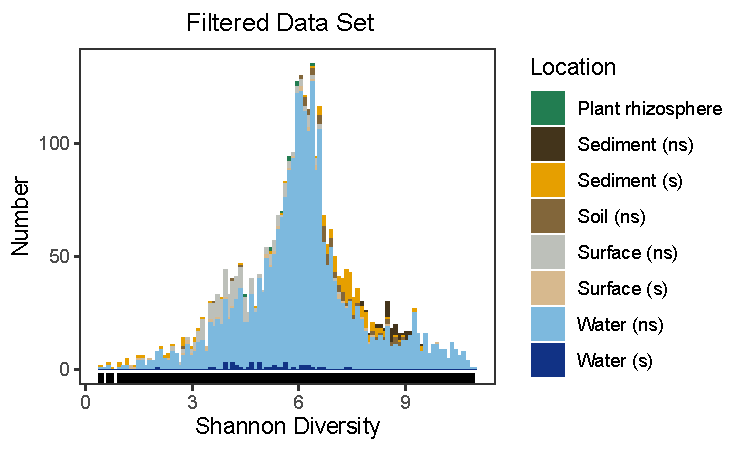
\includegraphics[scale=1]{./Figures/Filtered_Hist}
    \caption{\textbf{Distribution of bacterial diversity in the filtered data set for different EMPO3 categories.} All samples that don't have temperature and pH data are removed. Non-saline water samples (2529) have the highest number in the data set, followed by non-saline surface (195) and saline sediment (147). Here `ns' represents `non-saline' and `s' represents `saline'.}
    \label{fig:Filtered_Hist}
\end{figure}

\subsection{Bacterial diversity analysis}

All statistical analyses are conducted in the R V4.1.1 \citep{team2013r}. I calculated alpha diversity based on absolute species richness (observed OTUs), Chao1-estimated richness \citep{chao1984nonparametric}, and Shannon-Wiener index \citep{hill2003using} and formed a comparison of the three. At the same time, I calculate the phylogenetic diversity of the samples in the filtered data set to compare with the above three diversity indices with the R packages 'picante' \citep{kembel2010picante} and ‘vegan’ \citep{oksanen2013package}. Since there are some samples with missing data, I filtered the data set for analysing phylogenetic diversity, which contains 928 samples from 7 empo\_3 environments. I use the 'vegan' package \citep{oksanen2013package} for non-metric multidimensional scaling (NMDS) analysis and use its 'envfit' function to present environmental variables as explanatory variables.

\subsection{Model Fitting}

After judging that there is no apparent linear relationship between bacterial diversity and temperature, pH and latitude (Figure \ref{fig:Pairs}), I use polynomial regression models to fit the effects of environmental variables at different spatial scales on the microbial diversity index to predict the relationship between bacterial diversity and temperature, pH, and latitude with the R packages 'car' \citep{fox2012package} and 'randomForest' \citep{rcolorbrewer2018package}. According to the Akaike information criterion (AIC) criterion, the 'optimal model' is screened to determine the main driving factors, and the variance inflation factor (VIF) is used for collinearity diagnosis, and the variables with VIF \textless 10 are eliminated before refitting. 

I also use random forest modelling to investigate the impact of environmental factors, which is a robust method for improving predictive ability with large and and messy data sets containing nonlinear response-predictor relationships \citep{breiman2001random, cutler2007random}.  I utilise a percentage increase in the MSE (Mean Squared Error) of a variable to measure the importance of these diversity indices: a higher MSE per cent value indicates a more critical variable. The results were to determine the value of each environmental variable, which can choose the factor that has the most significant effect on bacterial diversity. Significance of the random forest models are assessed by using the 'A3' package \citep{fortmann2015package}. Similarly, the significance of each environmental variable is assessed with the 'rfPermute' package \citep{archer2016package}.

\section{Results}

\subsection{Relationship between bacterial diversity and environmental variables at the global scale}

After observing the models of diversity indices and environmental variables (Table \ref{tab:Shan_models}, \ref{tab:models}), I found that the differences between the diversity indices were not significant. Here, I use the Shannon-Wiener index as the premier index to present, which is the most generally used alpha diversity index that combines species richness and abundance. Then, I show the polynomial regression models and present the impact of a single environmental variable and two environmental variables on bacterial diversity (Figure \ref{fig:Shan_PM_simpleTpL}, \ref{fig:Shan_PM_2EVs}, \ref{fig:OO_PM_simpleTpL}, \ref{fig:OO_PM_2EVs}). When analysing the relationship between temperature and Shannon diversity, I found that bacterial diversity is the highest at around 6.3 \textdegree C (Figure \ref{fig:Shan_PM_simpleTpL} A) and in neutral environments (Figure \ref{fig:Shan_PM_simpleTpL} B). In the relationship between latitude and bacterial diversity, the Shannon diversity peaks in mid-latitudes (Figure \ref{fig:Shan_PM_simpleTpL} C). 


There is an interesting phenomenon among three kinds of models, whose results show that the $R^{2}$ of the latitude-dependent models are more significant than that of the models independent of it (Table \ref{tab:Shan_models}, \ref{tab:models}). The most considerable model $R^{2}$ in polynomial regression models is the model of temperature, pH, and latitude (including interactions) on diversity, while the pH one is the smallest. At the same time, the worst performance is the diversity and temperature/pH model. The results of the random forest models show the best results. Among them, latitude explains 40.49-49.63$\%$ of the diversity models, followed by temperature and latitude, pH, and latitude, and temperature, pH and latitude, while the temperature model has the most negligible $R^{2}$ (0.078-0.0835). 

\begin{table}
    \caption{{\bf The performance of polynomial and random forest models in determining the effect of environmental variables on bacterial community diversity.} The interaction effect of the three environmental variables is the most influential factor on diversity in polynomial models. Latitude performs best as a single environmental variable, and is even the best influencing factor in the random forest models.} 
     \centering
    \begin{tabular}{ m{0.9cm}<{\centering}m{4cm}<{\centering}m{4cm}<{\centering}} 
    \toprule
     $R^{2}$ & Polynomial Model & Random Forest Model \\
     \midrule
    T*p*L & 0.219 & 0.386 \\
    T*p & 0.12 & 0.235 \\
    T*L & 0.197 & 0.389 \\
    p*L & 0.159 & 0.383 \\
    T & 0.081 & 0.084 \\
    p & 0.07 & 0.159 \\
    L & 0.145 & 0.405 \\
    \bottomrule
    \end{tabular}    
    \label{tab:Shan_models}
\end{table}

\begin{figure}
    \centering
    \includegraphics[scale=0.8]{./Figures/Shan_PM_simpleTpL}
    \caption{\textbf{Effect of a single environmental variables on bacterial diversity at the global scale.} A-C: Polynomial regression models of diversity and temperature, pH and latitude ($R^{2}$=0.081, 0.07, 0.145). Diversity peaks at around 6.3 \textdegree C and pH around 6.6. Latitude performs best in these models.}
    \label{fig:Shan_PM_simpleTpL}
\end{figure}

\begin{figure}
    \centering
    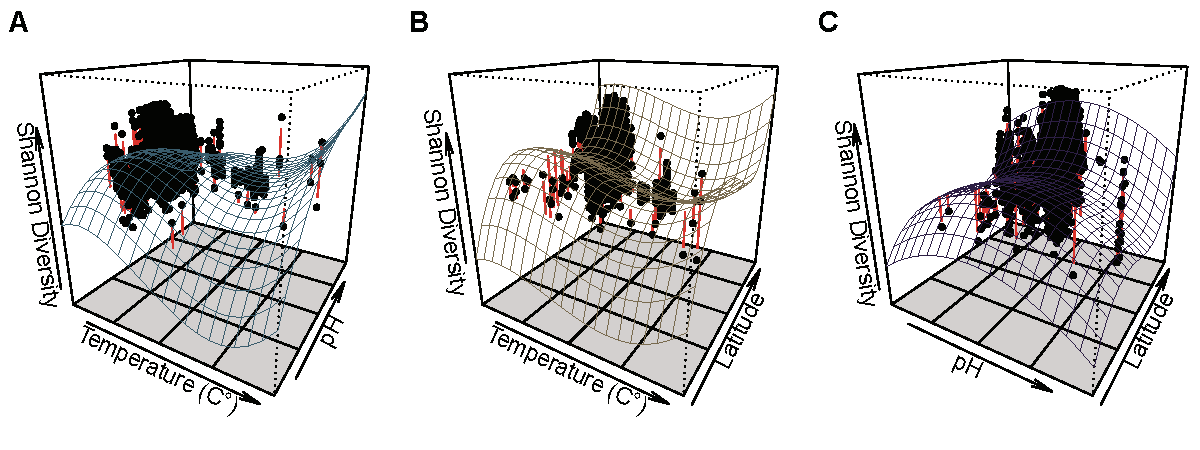
\includegraphics[scale=0.8]{./Figures/Shan_PM_all_2EVs_3D}
    \caption{\textbf{Effect of two environmental variables on bacterial diversity at the global scale.} A: Polynomial regression model of diversity versus temperature and pH ($R^{2}$=0.12). B: Model of diversity versus temperature and latitude ($R^{2}$=0.197). C: Model of diversity versus pH and latitude ($R^{2}$=0.159).}
    \label{fig:Shan_PM_2EVs}
\end{figure}

My EMPO3 model differed slightly from the overall sample in predicting bacterial diversity (Table \ref{tab:Shan_EMPO3models}). Polynomial regression models for the three EMPO3 environmental samples indicated that latitude was the single environmental variable with the most significant effect on diversity. In the non-saline water and non-saline surface environments, the combination of the three environmental variables was the most influential factor. However, in the saline sediment environment, the combination of variables was an inferior fit. Meanwhile, pH-related factors performed the worst in non-saline water and saline sediment environments. Overall, the random forest model was a better fit. However, as the sample size decreases, the fit of the random forest model decreases. For example, in the non-saline surface and saline sediment environments, the $R^{2}$ of some polynomial models was more significant than that of the random forest model. Latitude still performed best in the non-saline water environment. In the non-saline surface samples, the $R^{2}$ of the environmental variables did not vary significantly, except for latitude, which was less different. All environmental variables in the saline sediment samples explained the diversity to a similar extent.

\begin{table}
    \caption{{\bf The performance of models in determining the effect of environmental variables on bacterial diversity of EMPO3 categories.} In non-saline water environments, combinations of environmental variables in polynomial models perform better than single environmental variables. In contrast, random forest models with latitude have the most significant $R^{2}$. In the non-saline surface environment, combining the three environmental variables has the most significant effect on diversity. The latitude polynomial model $R^{2}$ is most significant, and all random forest models fit similarly for the saline sediment data set.}
    \centering
    \begin{tabular}{ m{3cm}<{\centering}m{2cm}<{\centering}m{4cm}<{\centering}m{4cm}<{\centering}} 
    \toprule
    Environment & $R^{2}$ & Polynomial Model & Random Forest Model \\
     \midrule
    \multirow{7}*{Non-saline Water} & T*p*L & 0.236 & 0.322 \\
    & T*p & 0.115 & 0.153 \\
    & T*L & 0.217 & 0.323 \\
    & p*L & 0.206 & 0.319 \\
    & T & 0.052 & NULL \\
    & p & 0.097 & 0.113 \\
    & L & 0.196 & 0.346 \\
    \midrule
    \multirow{7}*{Non-saline Surface} & T*p*L & 0.551 & 0.48 \\
    & T*p & 0.292 & 0.476 \\
    & T*L & 0.444 & 0.463 \\
    & p*L & 0.393 & 0.468 \\
    & T & 0.269 & 0.47 \\
    & p & 0.194 & 0.423 \\
    & L & 0.271 & 0.254 \\
    \midrule
    \multirow{7}*{Saline Sediment} & T*p*L & NULL & 0.404 \\
    & T*p & NULL & 0.394 \\
    & T*L & NULL & 0.399 \\
    & p*L & NULL & 0.399 \\
    & T & 0.149 & 0.39 \\
    & p & 0.107 & 0.385 \\
    & L & 0.41 & 0.4 \\
    \bottomrule
    \end{tabular}    
    \label{tab:Shan_EMPO3models}
\end{table}

The above patterns are also almost similar in absolute richness (observed OTUs) and Chao1 richness (\multiref{fig:Chao_PM_simpleTpL}{fig:OO_PM_2EVs}, Table \ref{tab:models}, \ref{tab:EMPO3models}). Even though the data set of phylogenetic diversity has some samples missing, I still observe results in it that don't differ significantly from other indices of diversity at the global scale (Figure \ref{fig:PD_PM_simpleTpL}, \ref{fig:PD_PM_2EVs}).

\subsection{Relationship between bacterial community diversity and environmental variables at the local scale}

The two models I selected from the three locations both show the same results (Figure \ref{fig:Shan_PM_local_1and2EVs}, Table \ref{tab:Shan_localmodels}, \ref{tab:localmodels}); that is, temperature and pH (including interactions) performed best in predicting bacterial diversity. While under the influence of a single environmental variable, the $R^{2}$ of the temperature models is basically more considerable than those of the pH models except for the Yellowstone samples, and even in some models, the relationships between pH and diversity indices are not significant. The random forest models also show better predictive performance than the polynomial regression models in the Yellowstone data set. However, the $R^{2}$ of the polynomial regression models is the largest in the Großer Stechlinsee and Toolik Lake data sets, indicating that the polynomial regression model is more able to detect weak trends. In the Yellowstone samples, the temperature and pH $R^{2}$ is not significantly different, which means that both variables significantly affect bacterial diversities. Due to insufficient samples containing phylogenetic diversity, small-scale effects on it are not analysed here. The above patterns are also almost similar in absolute richness (observed OTUs) and Chao1 richness (Figure \ref{fig:Chao_PM_local_1and2EVs}, \ref{fig:OO_PM_local_1and2EVs}, Table \ref{tab:localmodels}), with the models fitting the absolute richness somewhat better than the other two diversity indices.

\begin{table}
    \caption{{\bf The performance of models in determining the effect of environmental variables on bacterial community diversity at the local scale.} Location 1, 2 and 3 are Yellowstone National Park, Großer Stechlinsee and Toolik Lake respectively. The combination of temperature and pH performs better than a single variable in these three locations.}
    \centering
    \begin{tabular}{ m{1.5cm}<{\centering}m{4cm}<{\centering}m{4cm}<{\centering}} 
     \toprule
     $R^{2}$ & Polynomial Model & Random Forest Model \\
     \midrule
    L1 T*p & 0.315 & 0.481 \\
    L2 T*p & 0.049 & NULL \\
    L3 T*p & 0.053 & 0.01 \\
    L1 T & 0.267 & 0.472 \\
    L2 T & 0.01 & NULL \\
    L3 T & 0.049 & NULL \\
    L1 p & 0.289 & 0.427 \\
    L2 p & 0.036 & NULL \\
    L3 p & NULL & NULL \\
    \bottomrule
    \end{tabular}    
    \label{tab:Shan_localmodels}
\end{table}

\begin{figure}
    \centering
    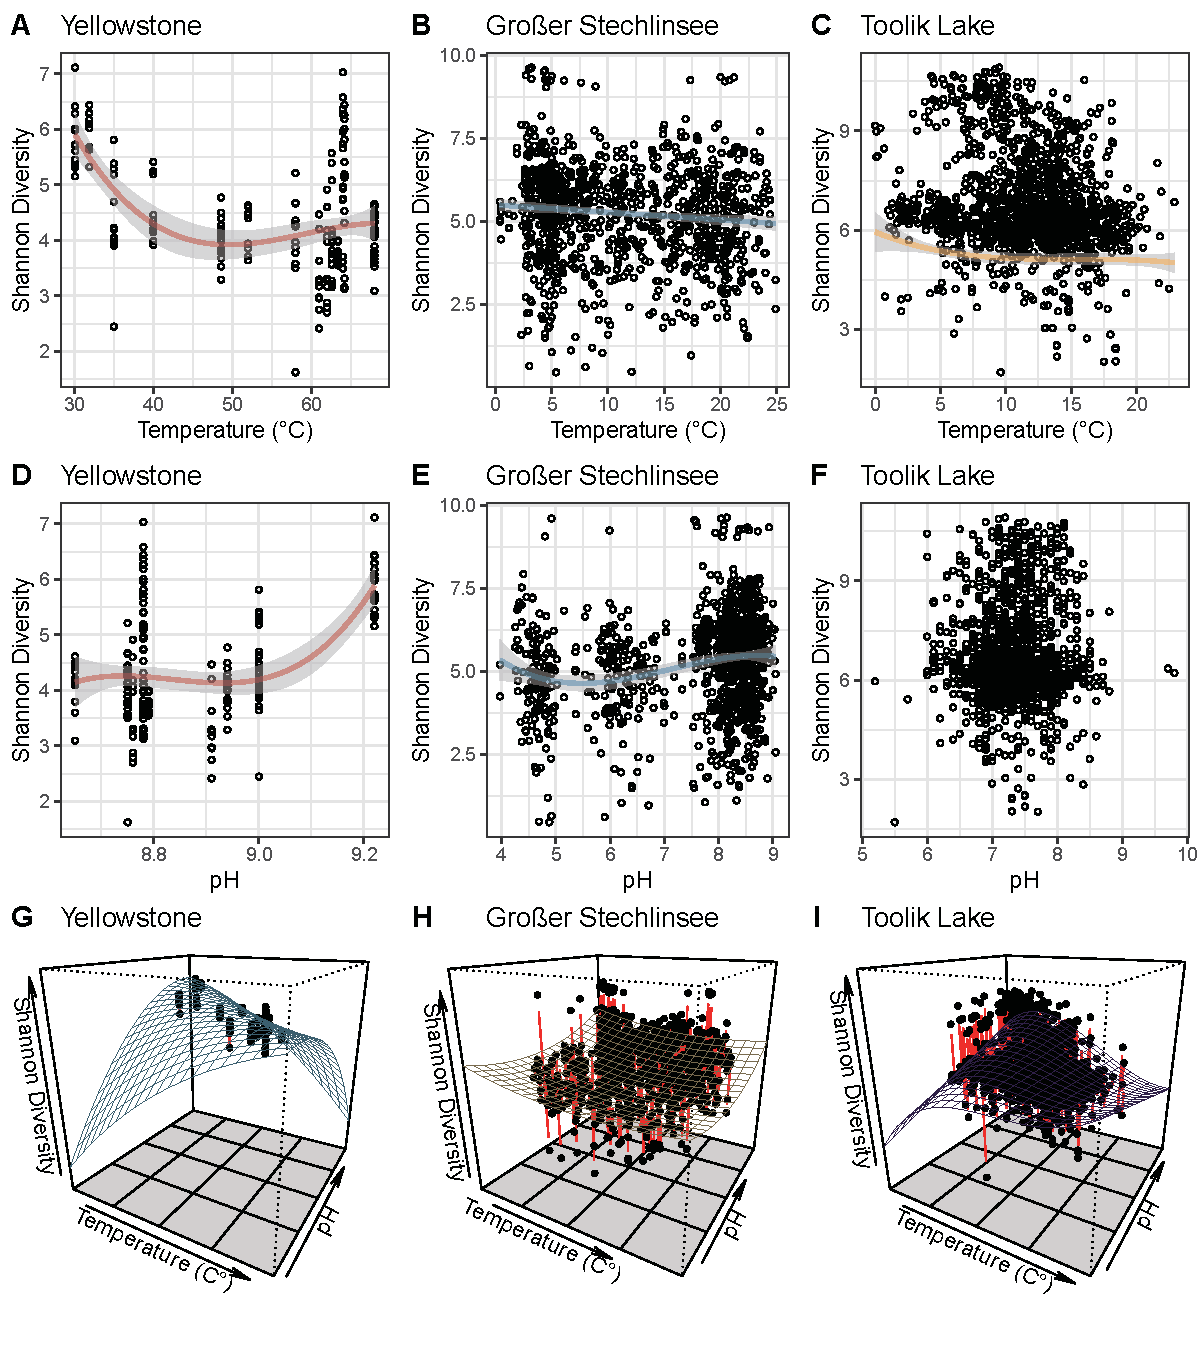
\includegraphics[scale=0.8]{./Figures/Shan_PM_local_1and2EVs_3D}
    \caption{\textbf{Effect of environmental variables on bacterial diversity at the local scale.} A-C: Polynomial regression models of diversity and temperature from three locations ($R^{2}$=0.267, 0.01, 0.049). D-E: Models of diversity and pH ($R^{2}$=0.289, 0.036). F: There is no significant relationship between pH and diversity in the Toolik Lake samples. These results indicate that even the $R^2$ values of temeprature models are generally low, temperature has always had some impact on diversity. G-I: Polynomial regression model of diversity versus temperature and pH from three locations ($R^{2}$=0.315, 0.049, 0.053). These results indicate that the combined effect of temperature and pH is slightly better than a single environmental variable at the local scale.}
    \label{fig:Shan_PM_local_1and2EVs}
\end{figure}

\section{Discussion}

To study the impact of environmental variables on bacterial diversity in a new global data set, I selected two of the most easily measurable environmental factors, temperature, pH, and I observed the effect of latitude. My findings suggest that latitude may best predict bacterial diversity at the global scale. While the combination of temperature and pH performed best at the local scale, temperature is strongly recommended if it is a single environmental variable. At the same time, the model fitting effect of the combination of environmental variables is basically better than that of a single variable, which shows that it cannot be ignored and disassembled.

The bacterial diversity peaked at around 6.3 \textdegree C in the filtered data set (Figure \ref{fig:Shan_PM_2EVs} A). Likewise, I look at the relationship between bacterial diversity and temperature for all samples in the data set with temperature data, and it turns out that bacterial diversity decreases with increasing temperature (Figure \ref{fig:Chao_T}, \ref{fig:OO_T}, \ref{fig:Shan_T}). The results from my models show that temperature is strongly associated with bacterial diversity at the global scales. Even though the results show that the $R^{2}$ of the temperature model of the Yellowstone data set is smaller than that of the pH model, the difference is not significant. At the same time, many of the pH-related models are very poor at fitting bacterial diversity, and most models between diversity and temperature show relevant results (Table \ref{tab:Shan_localmodels}). Therefore, temperature is an essential environmental predictor of bacterial diversity at the local scale. With global warming, climate change is causing changes in many ecosystem functions and will continue to do so for the next hundred years \citep{smith2018predicted}. Temperature, precipitation and extreme climate changes due to global warming may cause microbial communities to adapt to new conditions or alter the geographical distribution of microbes \citep{leducq2014local}. Due to the global change, factors affecting microbial communities may continue to change at regional and global scales. Much of the current research is based on easily observable targets such as plants and animals \citep{chen2011rapid, colwell2008global} and less on how 'cryptic' organisms like microbes respond to changes in temperature \citep{RePEc:nat:nature:v:463:y:2010:i:7279:d:10.1038_463293c}. Therefore, it is essential to study the 
patterns and mechanisms by which temperature regulates bacterial diversity. Temperature controls the chemical reaction rates and pathways of organisms \citep{birgander2018responses, dacal2019soil,walker2018microbial}, and it affects the growth rate of bacteria by affecting the thermal stability of proteins, thereby regulating biological pathways and mechanisms \citep{corkrey2012universality}. Changes in the rate of ecosystem processes ultimately depend on changes in the metabolic demands of individual organisms \citep{zhou2016temperature}.  There is currently insufficient research on the impact of temperature change on some fundamental characteristics of microbial communities, such as changes in microbial community diversity \citep{delgado2016microbial}, community composition, abundance \citep{maestre2015increasing}, and the role of microbes in controlling nutrient fluxes \citep{azam2007microbial, thornton2014dissolved}. In the future, the effect of temperature on the microbial community can be used as the main direction to continue research to further explore the changes in microbial community diversity with the temperature gradients.

My study shows that pH shows a similar degree of effect as temperature in partial models of Yellowstone samples and Großer Stechlinsee samples (Table \ref{tab:Shan_localmodels}), which indicates that pH also has an essential influence on bacterial diversity. With global climate change, many habitats around the world are experiencing significant changes in pH \citep{caldeira2003anthropogenic, cavicchioli2019scientists}. For instance, ${\rm CO_{2}}$ from the burning of chemical fuels can be absorbed by the upper water column and lead to an increase in pH \citep{houghton2001climate}, which is projected to decrease by a further 0.3–0.4 units by the end of the century \citep{hurd2018current} and the soil bacterial community, which is highly responsive to precipitation and pH \citep{bahram2018structure}, can be greatly affected. The decreasing pH may affect community metabolism, growth, and reproduction through intracellular pH homeostasis \citep{melzner2009physiological}. For instance, as ocean pH decreases, the energy required for bacterial cell maintenance increases rather than growth; the pH homeostatic mechanism takes up the majority of bacteria's transcriptional efforts, potentially affecting bacterial carbon cycling and energy fluxes in microbial food webs \citep{bunse2016response}. This may lead to ecological impacts through, for example, the disappearance of specific species, which may affect local biodiversity and lead to disturbances in community composition. In turn, changes in pH conditions can lead to changes in oxygen consumption \citep{bunse2016response}, metabolism \citep{arnosti2011dynamics, grossart2006testing}, and food response \citep{piontek2010acidification} of the microbiome.Supplemented by more research and data in the future, pH may play a more significant role in predicting microbial community diversity.

Geographical patterns of bacterial diversity may help people better understand the prevalence of microbial community patterns and the mechanisms in organisms that respond to environmental changes \citep{fuhrman2008latitudinal}. I observe the relationship between bacterial diversity and latitude for all samples, and the result is that bacterial diversity peaks in the subtropical to mid-latitude regions (Figure \ref{fig:Chao_lati}, \ref{fig:OO_lati}, \ref{fig:Shan_lati}). Similarly, the result of my filtered data set also exhibits the same pattern (Figure \ref{fig:Shan_PM_2EVs} C), which likely reflects the actual latitudinal diversity gradient from the equator to the poles. Latitude had the best effect on predicting bacterial diversity at the global scale. The latitudinal gradient is one of the oldest and most common biodiversity patterns worldwide, characterized by decreasing species diversity from the tropics to the poles \citep{gaston1996biodiversity, gaston2000global, stevens1989latitudinal}. Contrary to previous beliefs, a growing body of biogeographic research shows that whether animals, plants or bacteria have peaks in biodiversity in subtropical to temperate zones \citep{kerswell2006global, ladau2013global, lucifora2011global, phillips2019global, sato2021potential, tittensor2010global}. With global warming, climate change has led to changes in many ecosystem functions, with global mean surface temperature (GMST) increasing at a rate of 0.2° ± 0.1°C per decade \citep{change2007climate}. This has an enormous effect on tropical species \citep{antao2020temperature, colwell2008global, dillon2010global, pounds1999biological}, which have a narrower heat tolerance than temperate species, and which live at ambient temperatures very close to their physiological optimum \citep{deutsch2008impacts}. Warming could increase the abundance of many species that benefit from it and allow them to expand their geographic range \citep{chen2011rapid, hickling2006distributions, thomas2010climate}. Since most of the world's species are found in the tropics, warmer temperate regions at lower latitudes are likely to experience significantly higher species richness and increases in abundance \citep{bates2014defining, tittensor2010global}. And suitable environment may be why bacterial diversity peaks at the subtropical to mid-latitudes. Meanwhile, as the temperature increases, the metabolic rate of bacteria increases, and the carbon loss rate of some bacteria' respiration exceeds the carbon uptake rate, resulting in restricted growth \citep{smith2019community}. However, a small proportion of bacteria with high uptake rate and low respiration rate adapted to the higher temperature, and species resource utilisation ability increased with the increase of temperature. This may also explain why bacterial diversity is not high in tropical regions with higher temperatures. In contrast, In previous studies, studies along latitudinal gradients have generally considered temperature change as a driving variable of latitudinal change \citep{fierer2011microbes, gaston2000global}, however in this EMP dataset I adapted, sampling temperatures does not have a linear relationship with latitude (Figure \ref{fig:Pairs}). According to current research, latitudinal diversity is influenced by five primary elements: sampling effort \citep{fierer2011microbes}, climate \citep{currie1991energy, hawkins2003energy}, spatial characteristics (such as area) \citep{rosenzweig_1995, terborgh1973notion}, biological interactions (such as competition and symbiosis), and evolutionary tendencies \citep{gaston2000global, willig2003latitudinal}, while factors such as climate stability, environmental stability, environmental predictability, seasonality and harshness, are all incorporated \citep{kaufman1998structure, willig2003latitudinal}. Latitude patterns are like any complex system \citep{10011263723}, which combines many factors besides temperature and pH, so it's unlikely that any single variable will fully explain how species diversity occurs. Therefore, viewing latitude as an integrated mechanism of multiple factors may aplly to most biodiversity analyses \citep{gaston2000global, willig2003latitudinal}.

It can be observed in my findings that the $R^{2}$ of a polynomial regression model for a combination of three environmental variables is always greater than that of a model for a single variable (Table \ref{tab:models}, \ref{tab:localmodels}, \ref{tab:EMPO3models}). Other models exhibit this feature except for the random forest model of global-scale samples, which can indicate that the combination of multiple environmental factors significantly impacts bacterial community diversity and can more comprehensively display the law of diversity changes. At the same time, latitude as an environmental variable itself can also be regarded as a comprehensive mechanism composed of multiple factors. That is to say when analysing the impact of environmental variables on diversity, the effect of individual variables is still essential, but the combined effect needs to be considered more.

My random forest models show promising results when fitting samples with larger sample sizes. The polynomial regression model demonstrates a visualisation of trends in bacterial diversity in response to environmental variables. Almost all random forest models perform better than polynomial regression, with its best-fitting model having twice as much $R^{2}$ as the polynomial model. Also when the sample size is relatively small, the polynomial model may fit better than the random forest model. As discussed above, although I found some patterns in the variation of bacterial diversity with environmental gradients, these results cover only part of the bacterial habitat and environmental variables. While feasible in the EMP data set, the diversity gradients we observe necessarily reflect only a subset of the sample types in which the variable is measured, with the present difference of diverse and unmeasurable diversity of biotic or abiotic variables in different samples. The filtered data sets containing temperature and pH data are only one-eighth the size of the initial data sets. I also looked at community composition in the filtered data set, but the result shows slightly higher sample repeatability (Figure \ref{fig:nmds}). At the same time, the number of samples in each environment is not completely average, which may lead to the existence of the pattern of some environments that dominate the pattern of the entire data set (e.g. non-saline water samples occupy more than half of the filtered data set). The lack of data on bacteria in some common environments also led to some bias in my analysis. For example, soil bacteria, which play an essential role in the global carbon cycle \citep{reay2007greenhouse}, and marine bacteria, which are crucial in the nitrogen cycle \citep{halm2012heterotrophic}, are very common, which lack data on temperature and pH. Due to the absence of other environmental variables in the data set. Many important environmental factors are not considered while analysing. For example, salinity may be the most important environmental factor affecting global bacterial diversity \citep{lozupone2007global}; pH has the most critical influence on bacteria in many environments \citep{bunse2016response, fierer2006diversity,fierer2011microbes}; the impact of climatic conditions and global change factors on bacterial diversity has also received more and more attention \citep{drenovsky2010land, picazo2020climate, scherrer2010infra, zhou2020meta}. Understanding how these characteristics impact the worldwide distribution of bacteria might be crucial for humans to understand global biodiversity development and maintenance processes.

\section{Conclusion}

Improving understanding of global microbial biodiversity is one of the most important goals of contemporary ecologists. Even though the effect of a combination of environmental variables may not have the most potent influence in all cases, it has a more significant advantage than a single variable in most cases. My study suggests that latitude may be the most important environmental variable affecting bacterial diversity at the global scale and that bacterial diversity peaks at the subtropic to mid-latitudes. The combination of temperature and pH performed best at the local scale, and the temperature is most strongly associated with bacterial diversity as a single environmental variable. While these data do not fully cover all environmental variables, given that many environments are more difficult to measure other than temperature, pH, and geography, my study provides patterns about how microbial diversity varies with some fundamental environmental gradients and emphasises the scale-dependence of microbial diversity.

\section*{Code Availability}
\addcontentsline{toc}{section}{Code Availability}

The R code for models and analysis in this study is availible at my github (\href{https://github.com/ChuxuanJi/EECProject1}{\color{blue}{\underline{Chuxuan Ji EEC Project}}}) repository.

\section*{Acknowledgement}
\addcontentsline{toc}{section}{Acknowledgement}

I would like to express my greatest gratitude to Dr. Samraat Pawar for all his support and supervision throughout the entire project, even after his sabbatical started. I'm also sincerely grateful for all the inspiring ideas and thoughts Danica Duan (PhD candidate) and Dr. Tom Clegg provided throughout my project. And thank all three of them for providing feedback on my drafting thesis. I am very grateful to my parents, family and good friends for their great support and encouragement, and I am also very grateful to my girlfriend Xu Lan for her company across the ocean. In the end, I am also very grateful that I can continue to work hard in the direction I like. Every late night in front of the computer is an improvement for myself, and I hope that I can keep this spirit forever. 

\addcontentsline{toc}{section}{References}
\bibliographystyle{agsm}
\bibliography{thesis}
\clearpage


\begin{document}
\renewcommand{\thefigure}{SI.\arabic{figure}}
\setcounter{figure}{0}

\renewcommand{\thetable}{SI.\arabic{table}}
\setcounter{table}{0}

\section*{Supplementary Information}\label{sec:SI}

\addcontentsline{toc}{section}{Supplementary Information}
\addtocontents{toc}{\setcounter{tocdepth}{-10}}
\renewcommand{\thesubsection}{SI.\arabic{subsection}}
\setcounter{subsection}{0}


\subsection{Shannon Index and Observed OTUs plot}



\begin{figure}[H]
    \centering
    \includegraphics[scale=0.33]{./Figures/Chao_hist_empo3}
    \caption{\textbf{Distribution of Alpha Diversity in the empo\_3 samples.} A: Distribution of Chao1 index values for soil samples (4279 samples). B: Distribution of Chao1 index values for non-saline sediment samples (544 samples). C: Distribution of Chao1 index values for non-saline surface samples (1271 samples). D: Distribution of Chao1 index values for non-saline water samples (4915 samples). E: Distribution of Chao1 index values for saline sediment samples (559 samples). F: Distribution of Chao1 index values for saline surface samples (117 samples). G: Distribution of Chao1 index values for saline water samples (684 samples). H: Distribution of Chao1 index values for plant rhizosphere samples (554 samples). I: Distribution of Chao1 index values for plant surface samples (1611 samples). J: Distribution of Chao1 index values for plant corpus samples (125 samples). K: Distribution of Chao1 index values for animal secretion samples (1257 samples). L: Distribution of Chao1 index values for animal surface samples (2961 samples). M: Distribution of Chao1 index values for animal corpus samples (328 samples). N: Distribution of Chao1 index values for animal distal gut samples (4158 samples). O: Distribution of Chao1 index values for animal proximal gut samples (367 samples).}
    \label{fig:Chao_hist3}
\end{figure}

\begin{figure}[H]
    \centering
    \includegraphics[scale=0.33]{./Figures/Chao_lati_empo3}
    \caption{\textbf{The relationship between Chao1 index and latitude.} A: Trend of Chao1 index with latitude for soil samples. B: Trend of Chao1 index with latitude for non-saline water (water and sediment) samples. C: Trend of Chao1 index with latitude for saline water (water and sediment) samples. D: Trend of Chao1 index with latitude for non-saline sediment samples. E: Trend of Chao1 index with latitude for non-saline surface samples. F: Trend of Chao1 index with latitude for non-saline water samples. G: Trend of Chao1 index with latitude for saline sediment samples. H: Trend of Chao1 index with latitude for saline surface samples. I: Trend of Chao1 index with latitude for saline water samples. J: Trend of Chao1 index with latitude for animal surface samples. K: Trend of Chao1 index with latitude for plant surface samples. L: Trend of Chao1 index with latitude for plant rhizosphere samples.}
    \label{fig:Chao_lati3}
\end{figure}

\begin{figure}[H]
    \centering
    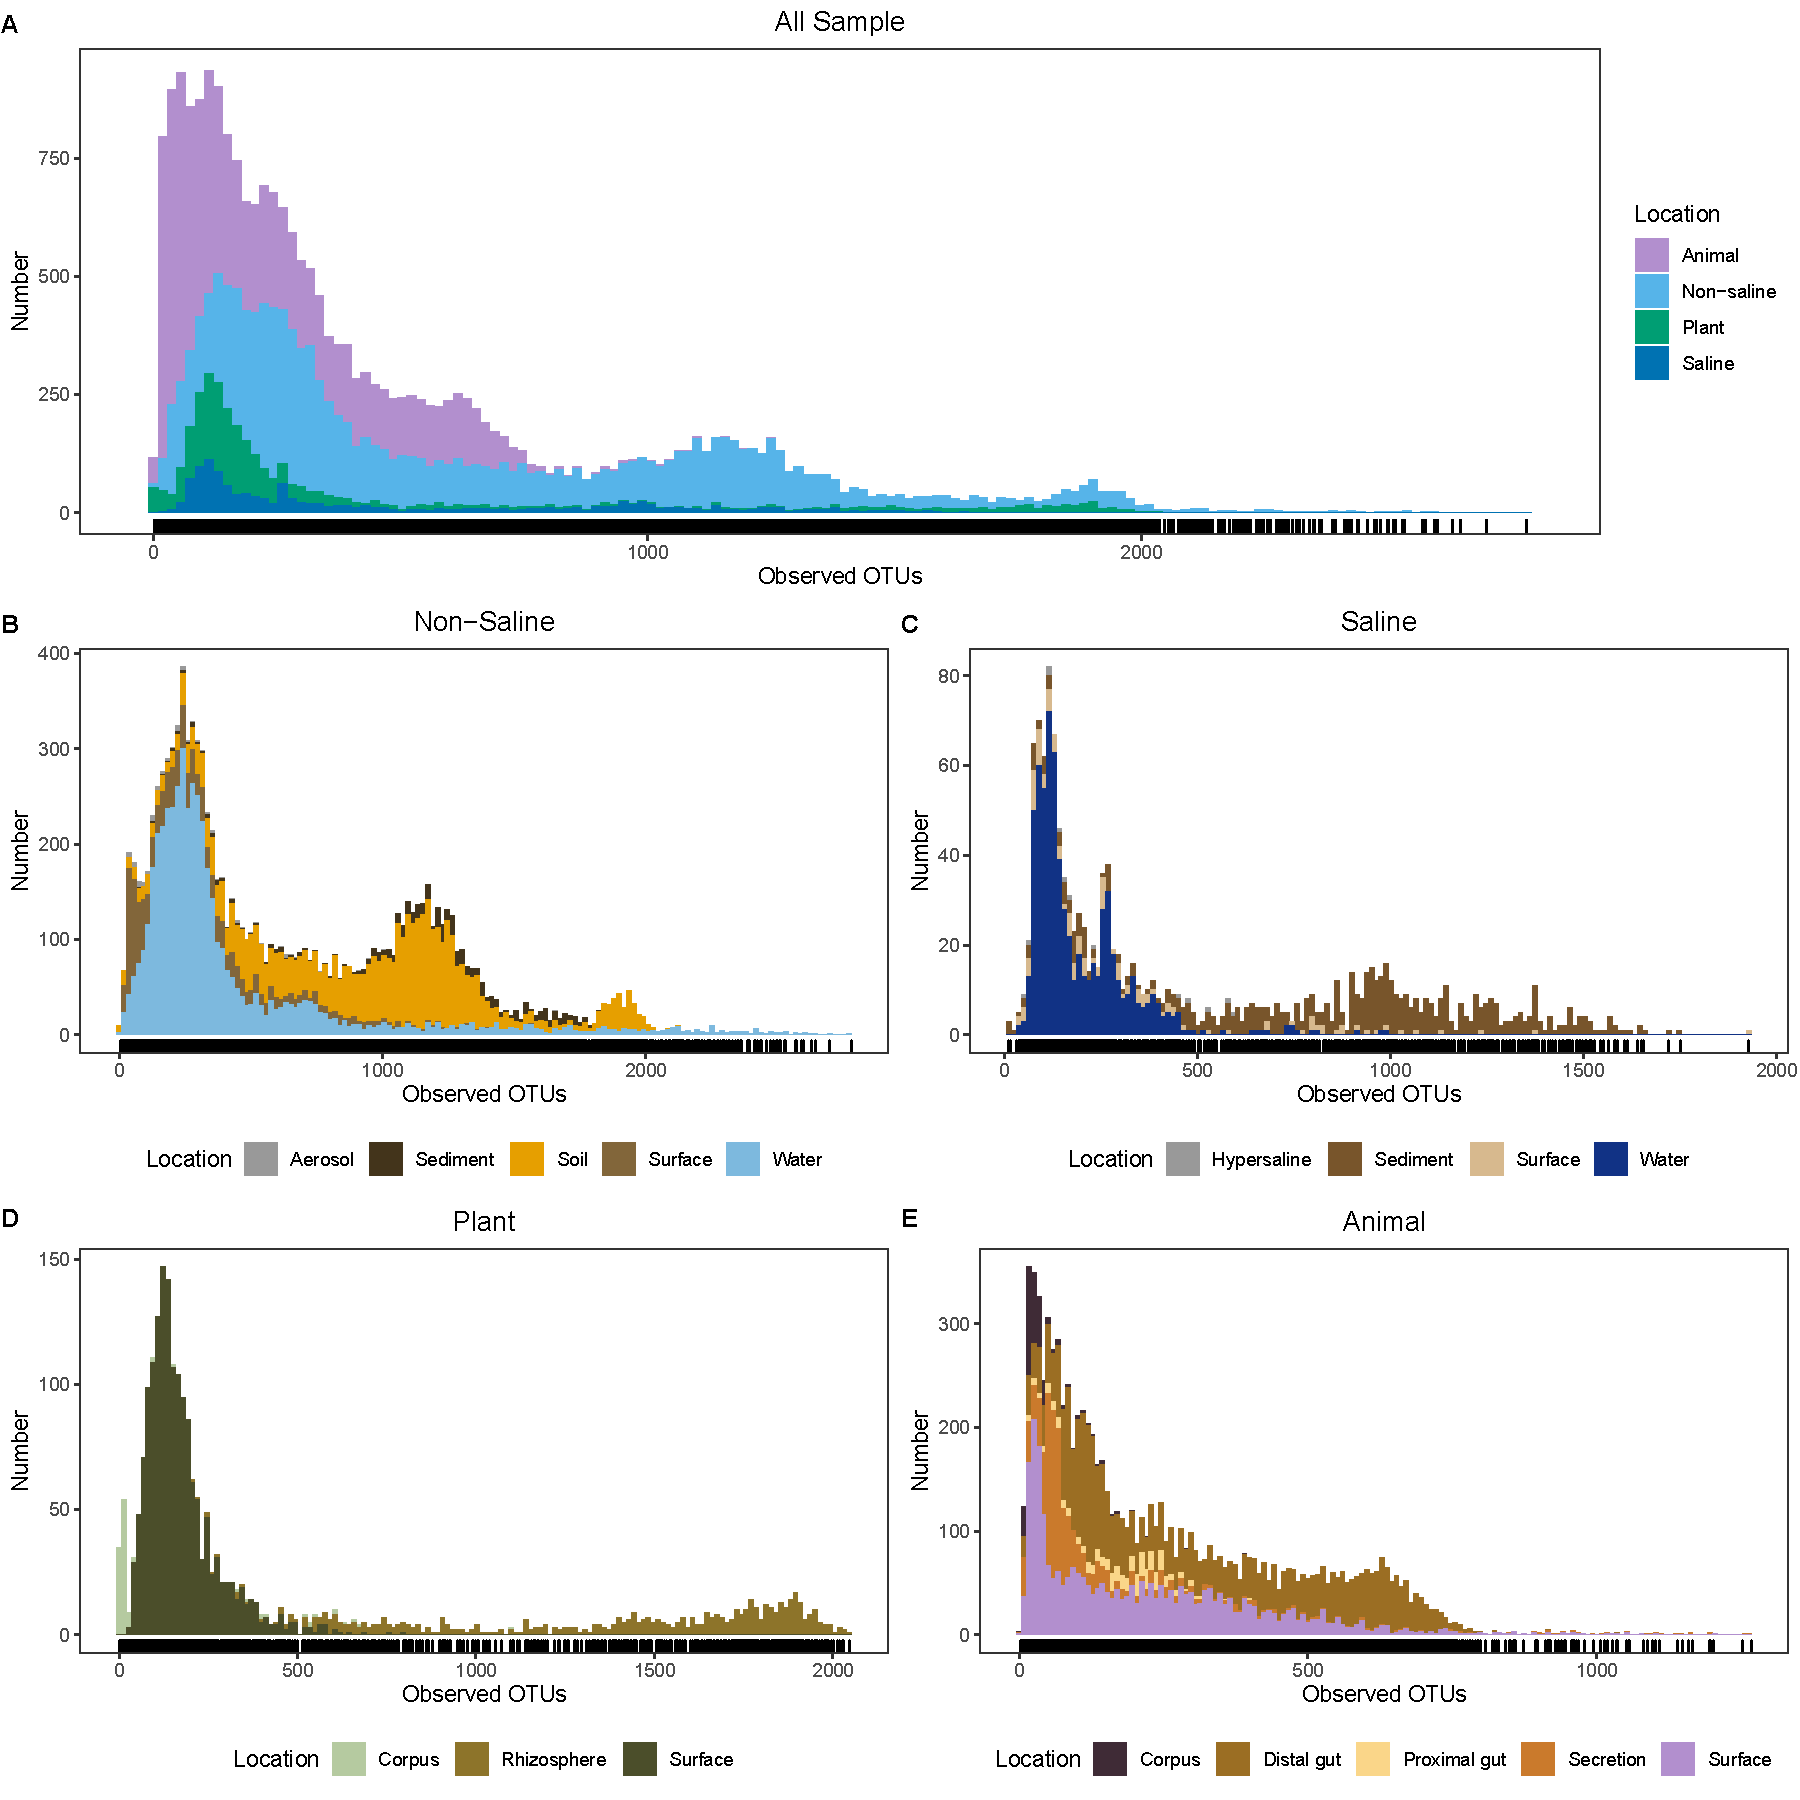
\includegraphics[scale=0.33]{./Figures/OO_hist_empo2}
    \caption{\textbf{Distribution of Observed OTUs in the whole dataset.} A: Distribution of Observed OTUs in the total dataset (23,820 samples, bin=150). B: Distribution of Observed OTUs for non-saline samples (11094 samples, bin=150). C: Distribution of Observed OTUs for saline samples (1373 samples, bin=150). D: Distribution of Observed OTUs for plant samples (2290 samples, bin=150). E: Distribution of Observed OTUs for animal samples (9071 samples, bin=150).}
    \label{fig:OO_hist}
\end{figure}

\begin{figure}[H]
    \centering
    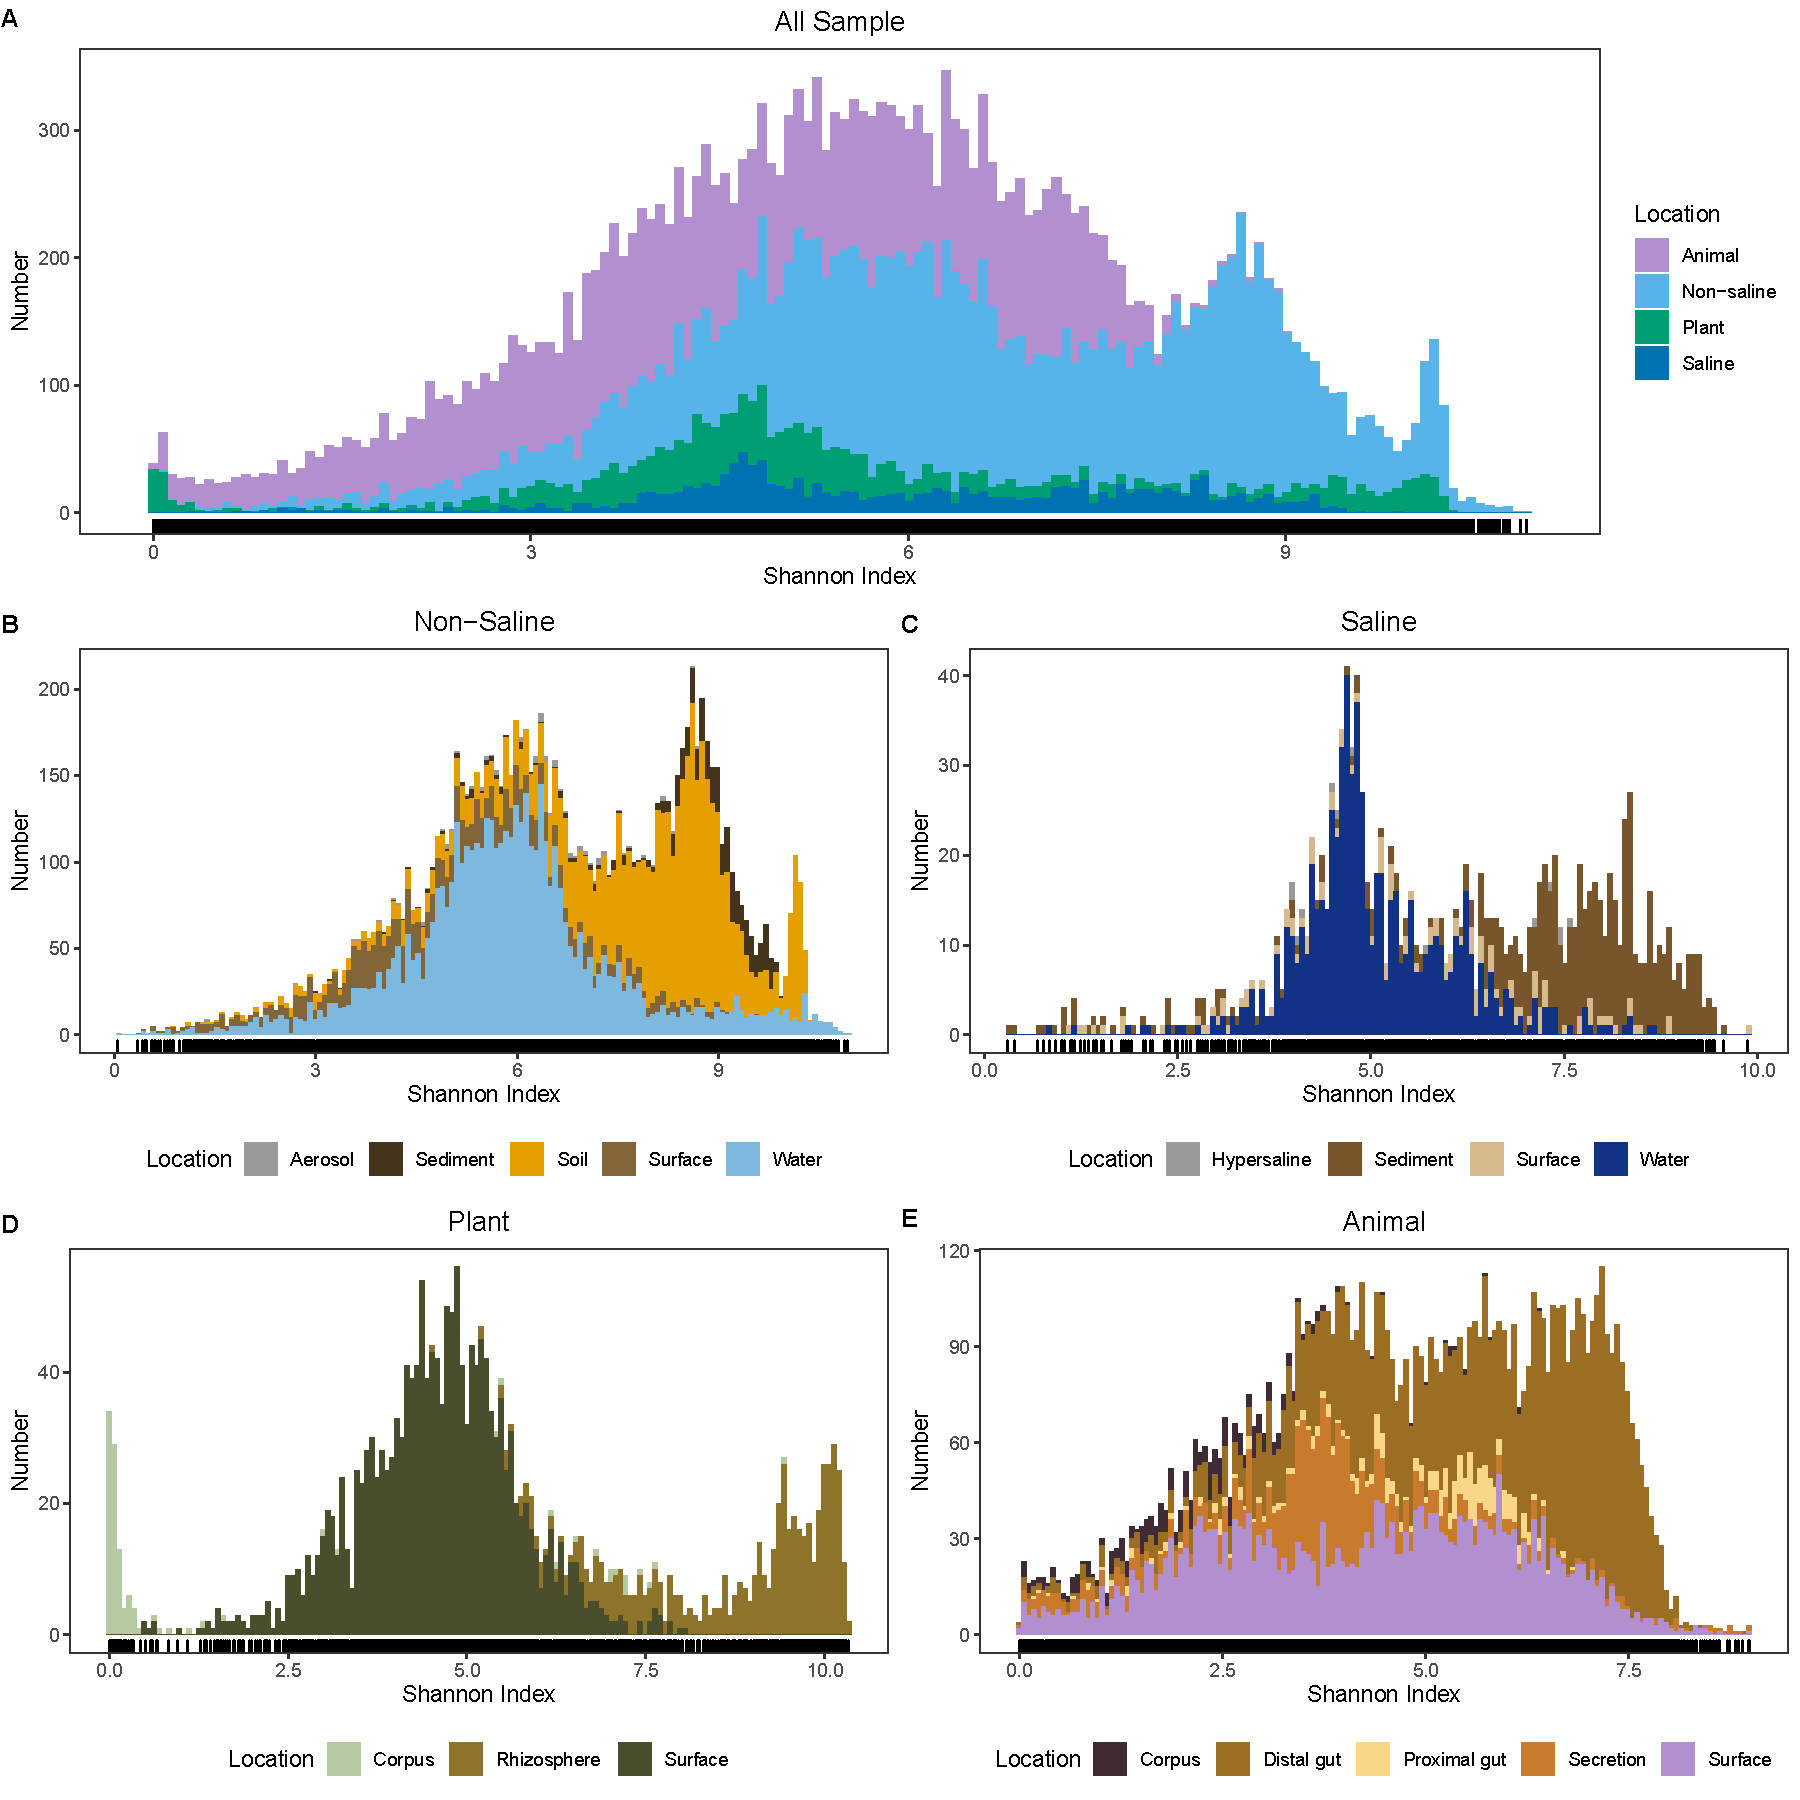
\includegraphics[scale=0.33]{./Figures/Shan_hist_empo2}
    \caption{\textbf{Distribution of Shannon index in the whole dataset.} A: Distribution of Shannon index values in the total dataset (23,820 samples, bin=150). B: Distribution of Shannon index values for non-saline samples (11094 samples, bin=150). C: Distribution of Shannon index values for saline samples (1373 samples, bin=150). D: Distribution of Shannon index values for plant samples (2290 samples, bin=150). E: Distribution of Shannon index values for animal samples (9071 samples, bin=150).}
    \label{fig:Shan_hist}
\end{figure}

\begin{figure}[H]
    \centering
    \includegraphics[scale=0.33]{./Figures/OO_hist_empo3}
    \caption{\textbf{Distribution of observed OTUs in the empo\_3 samples.} A: Distribution of observed OTUs for soil samples (4279 samples). B: Distribution of observed OTUs for non-saline sediment samples (544 samples). C: Distribution of observed OTUs for non-saline surface samples (1271 samples). D: Distribution of observed OTUs for non-saline water samples (4915 samples). E: Distribution of observed OTUs for saline sediment samples (559 samples). F: Distribution of observed OTUs for saline surface samples (117 samples). G: Distribution of observed OTUs for saline water samples (684 samples). H: Distribution of observed OTUs for plant rhizosphere samples (554 samples). I: Distribution of observed OTUs for plant surface samples (1611 samples). J: Distribution of observed OTUs for plant corpus samples (125 samples). K: Distribution of observed OTUs for animal secretion samples (1257 samples). L: Distribution of observed OTUs for animal surface samples (2961 samples). M: Distribution of observed OTUs for animal corpus samples (328 samples). N: Distribution of observed OTUs for animal distal gut samples (4158 samples). O: Distribution of observed OTUs for animal proximal gut samples (367 samples).}
    \label{fig:OO_hist3}
\end{figure}

\begin{figure}[H]
    \centering
    \includegraphics[scale=0.33]{./Figures/Shan_hist_empo3}
    \caption{\textbf{Distribution of Shannon index in the empo\_3 samples.} A: Distribution of Shannon index values for soil samples (4279 samples). B: Distribution of Shannon index values for non-saline sediment samples (544 samples). C: Distribution of Shannon index values for non-saline surface samples (1271 samples). D: Distribution of Shannon index values for non-saline water samples (4915 samples). E: Distribution of Shannon index values for saline sediment samples (559 samples). F: Distribution of Shannon index values for saline surface samples (117 samples). G: Distribution of Shannon index values for saline water samples (684 samples). H: Distribution of Shannon index values for plant rhizosphere samples (554 samples). I: Distribution of Shannon index values for plant surface samples (1611 samples). J: Distribution of Shannon index values for plant corpus samples (125 samples). K: Distribution of Shannon index values for animal secretion samples (1257 samples). L: Distribution of Shannon index values for animal surface samples (2961 samples). M: Distribution of Shannon index values for animal corpus samples (328 samples). N: Distribution of Shannon index values for animal distal gut samples (4158 samples). O: Distribution of Shannon index values for animal proximal gut samples (367 samples).}
    \label{fig:Shan_hist3}
\end{figure}

\begin{figure}[H]
    \centering
    \includegraphics[scale=0.33]{./Figures/OO_T_empo2}
    \caption{\textbf{The relationship between observed OTUs and temperature.} A: Trend of observed OTUs with temperature for samples in the whole dataset. B: Trend of observed OTUs with temperature for non-saline samples. C: Trend of observed OTUs with temperature for saline samples. D: Trend of observed OTUs with temperature for plant samples.}
    \label{fig:OO_T}
\end{figure}

\begin{figure}[H]
    \centering
    \includegraphics[scale=0.33]{./Figures/Shan_T_empo2}
    \caption{\textbf{The relationship between Shannon index and temperature.} A: Trend of Shannon index with temperature for samples in the whole dataset. B: Trend of Shannon index with temperature for non-saline samples. C: Trend of Shannon index with temperature for saline samples. D: Trend of Shannon index with temperature for plant samples.}
    \label{fig:Shan_T}
\end{figure}


\begin{figure}[H]
    \centering
    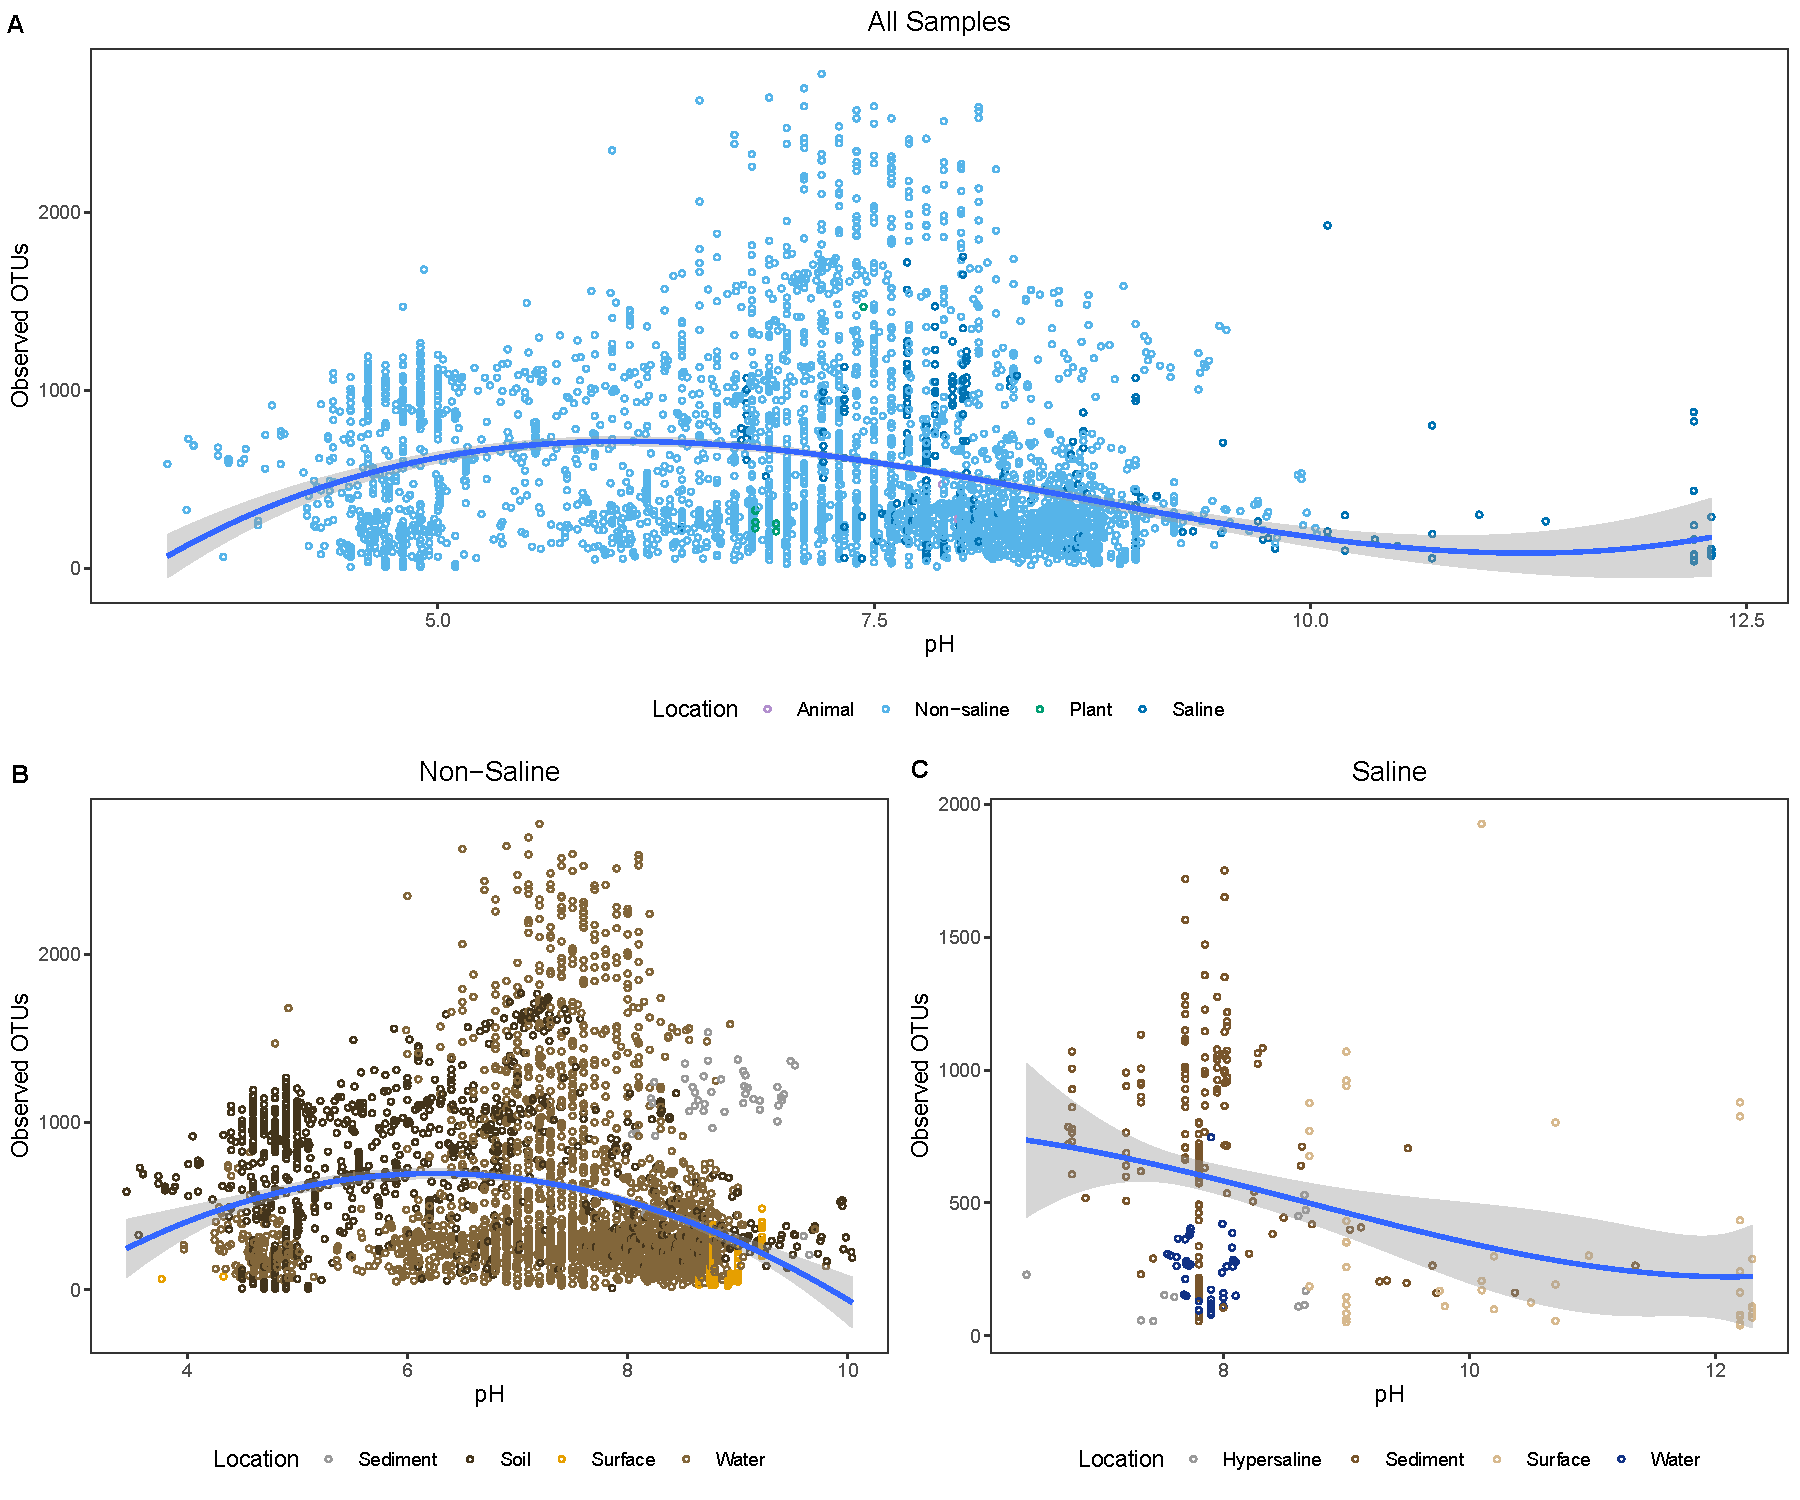
\includegraphics[scale=0.33]{./Figures/OO_pH_empo2}
    \caption{\textbf{The relationship between observed OTUs and pH.} A: Trend of observed OTUs with pH for samples in the whole dataset. B: Trend of observed OTUs with pH for non-saline samples. C: Trend of observed OTUs with pH for saline samples.}
    \label{fig:OO_pH}
\end{figure}

\begin{figure}[H]
    \centering
    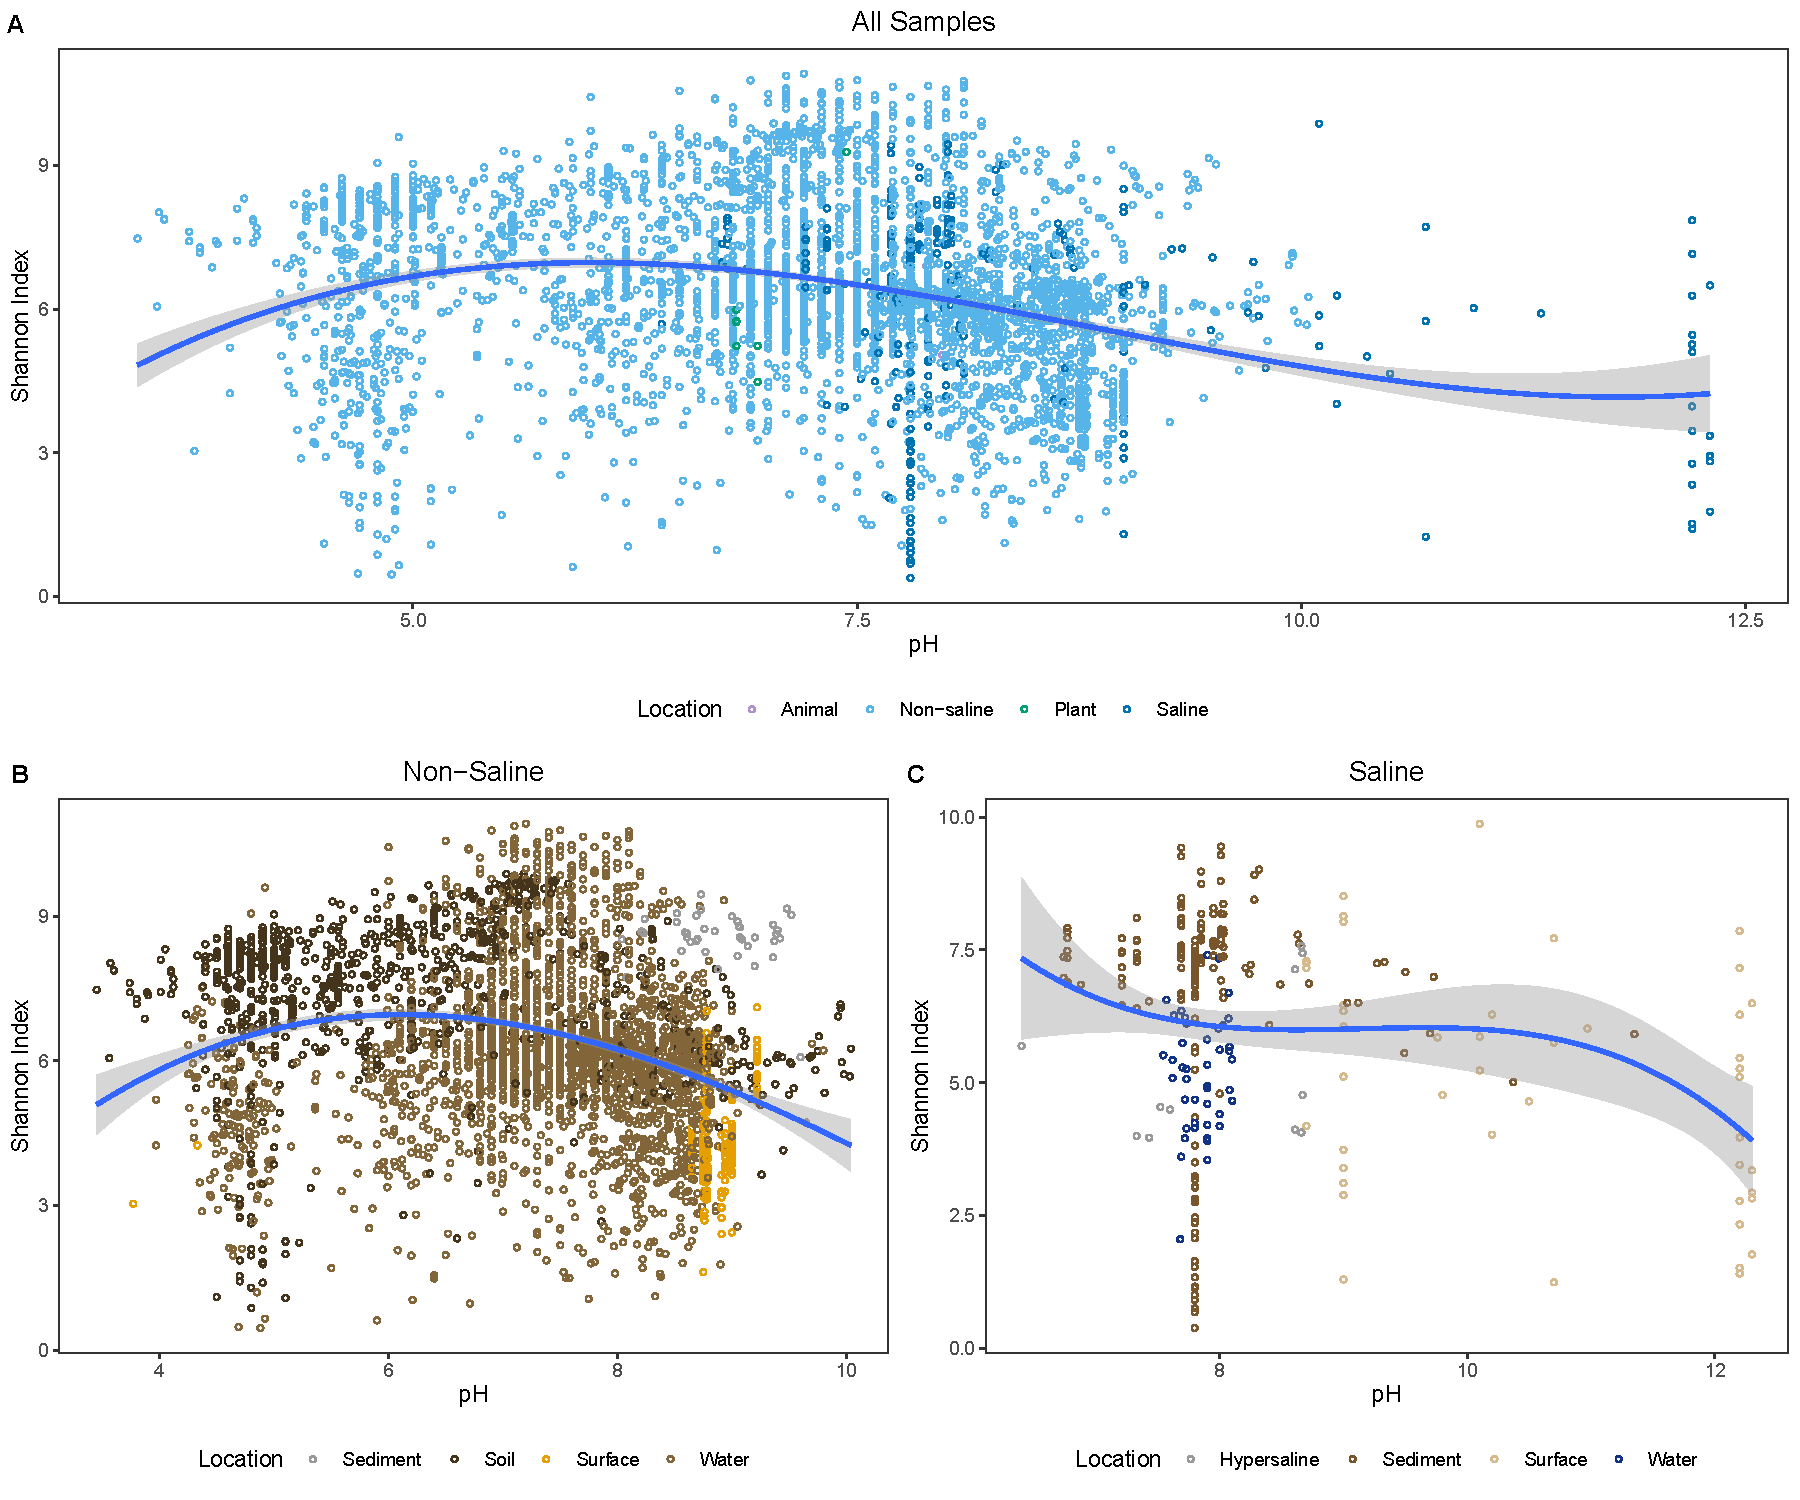
\includegraphics[scale=0.33]{./Figures/Shan_pH_empo2}
    \caption{\textbf{The relationship between Shannon index and pH.} A: Trend of Shannon index with pH for samples in the whole dataset. B: Trend of Shannon index with pH for non-saline samples. C: Trend of Shannon index with pH for saline samples.}
    \label{fig:Shan_pH}
\end{figure}

\begin{figure}[H]
    \centering
    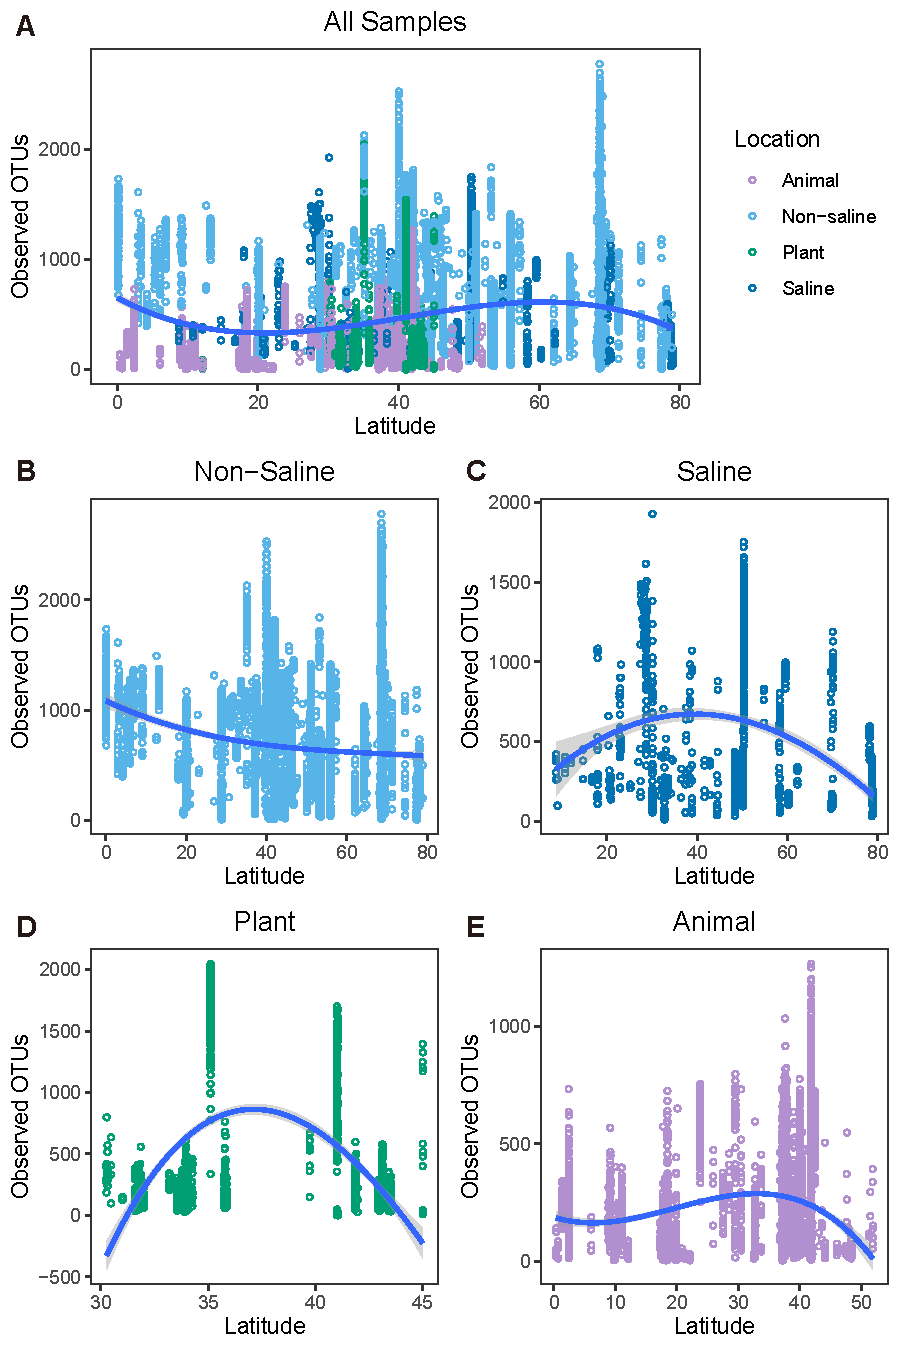
\includegraphics[scale=0.33]{./Figures/OO_lati_empo2}
    \caption{\textbf{The relationship between observed OTUs and latitude.} A: Trend of observed OTUs with latitude for samples in the whole dataset. B: Trend of observed OTUs with latitude for non-saline samples. C: Trend of observed OTUs with latitude for saline samples. D: Trend of observed OTUs with latitude for plant samples. E: Trend of observed OTUs with latitude for animal samples.}
    \label{fig:OO_lati}
\end{figure}

\begin{figure}[H]
    \centering
    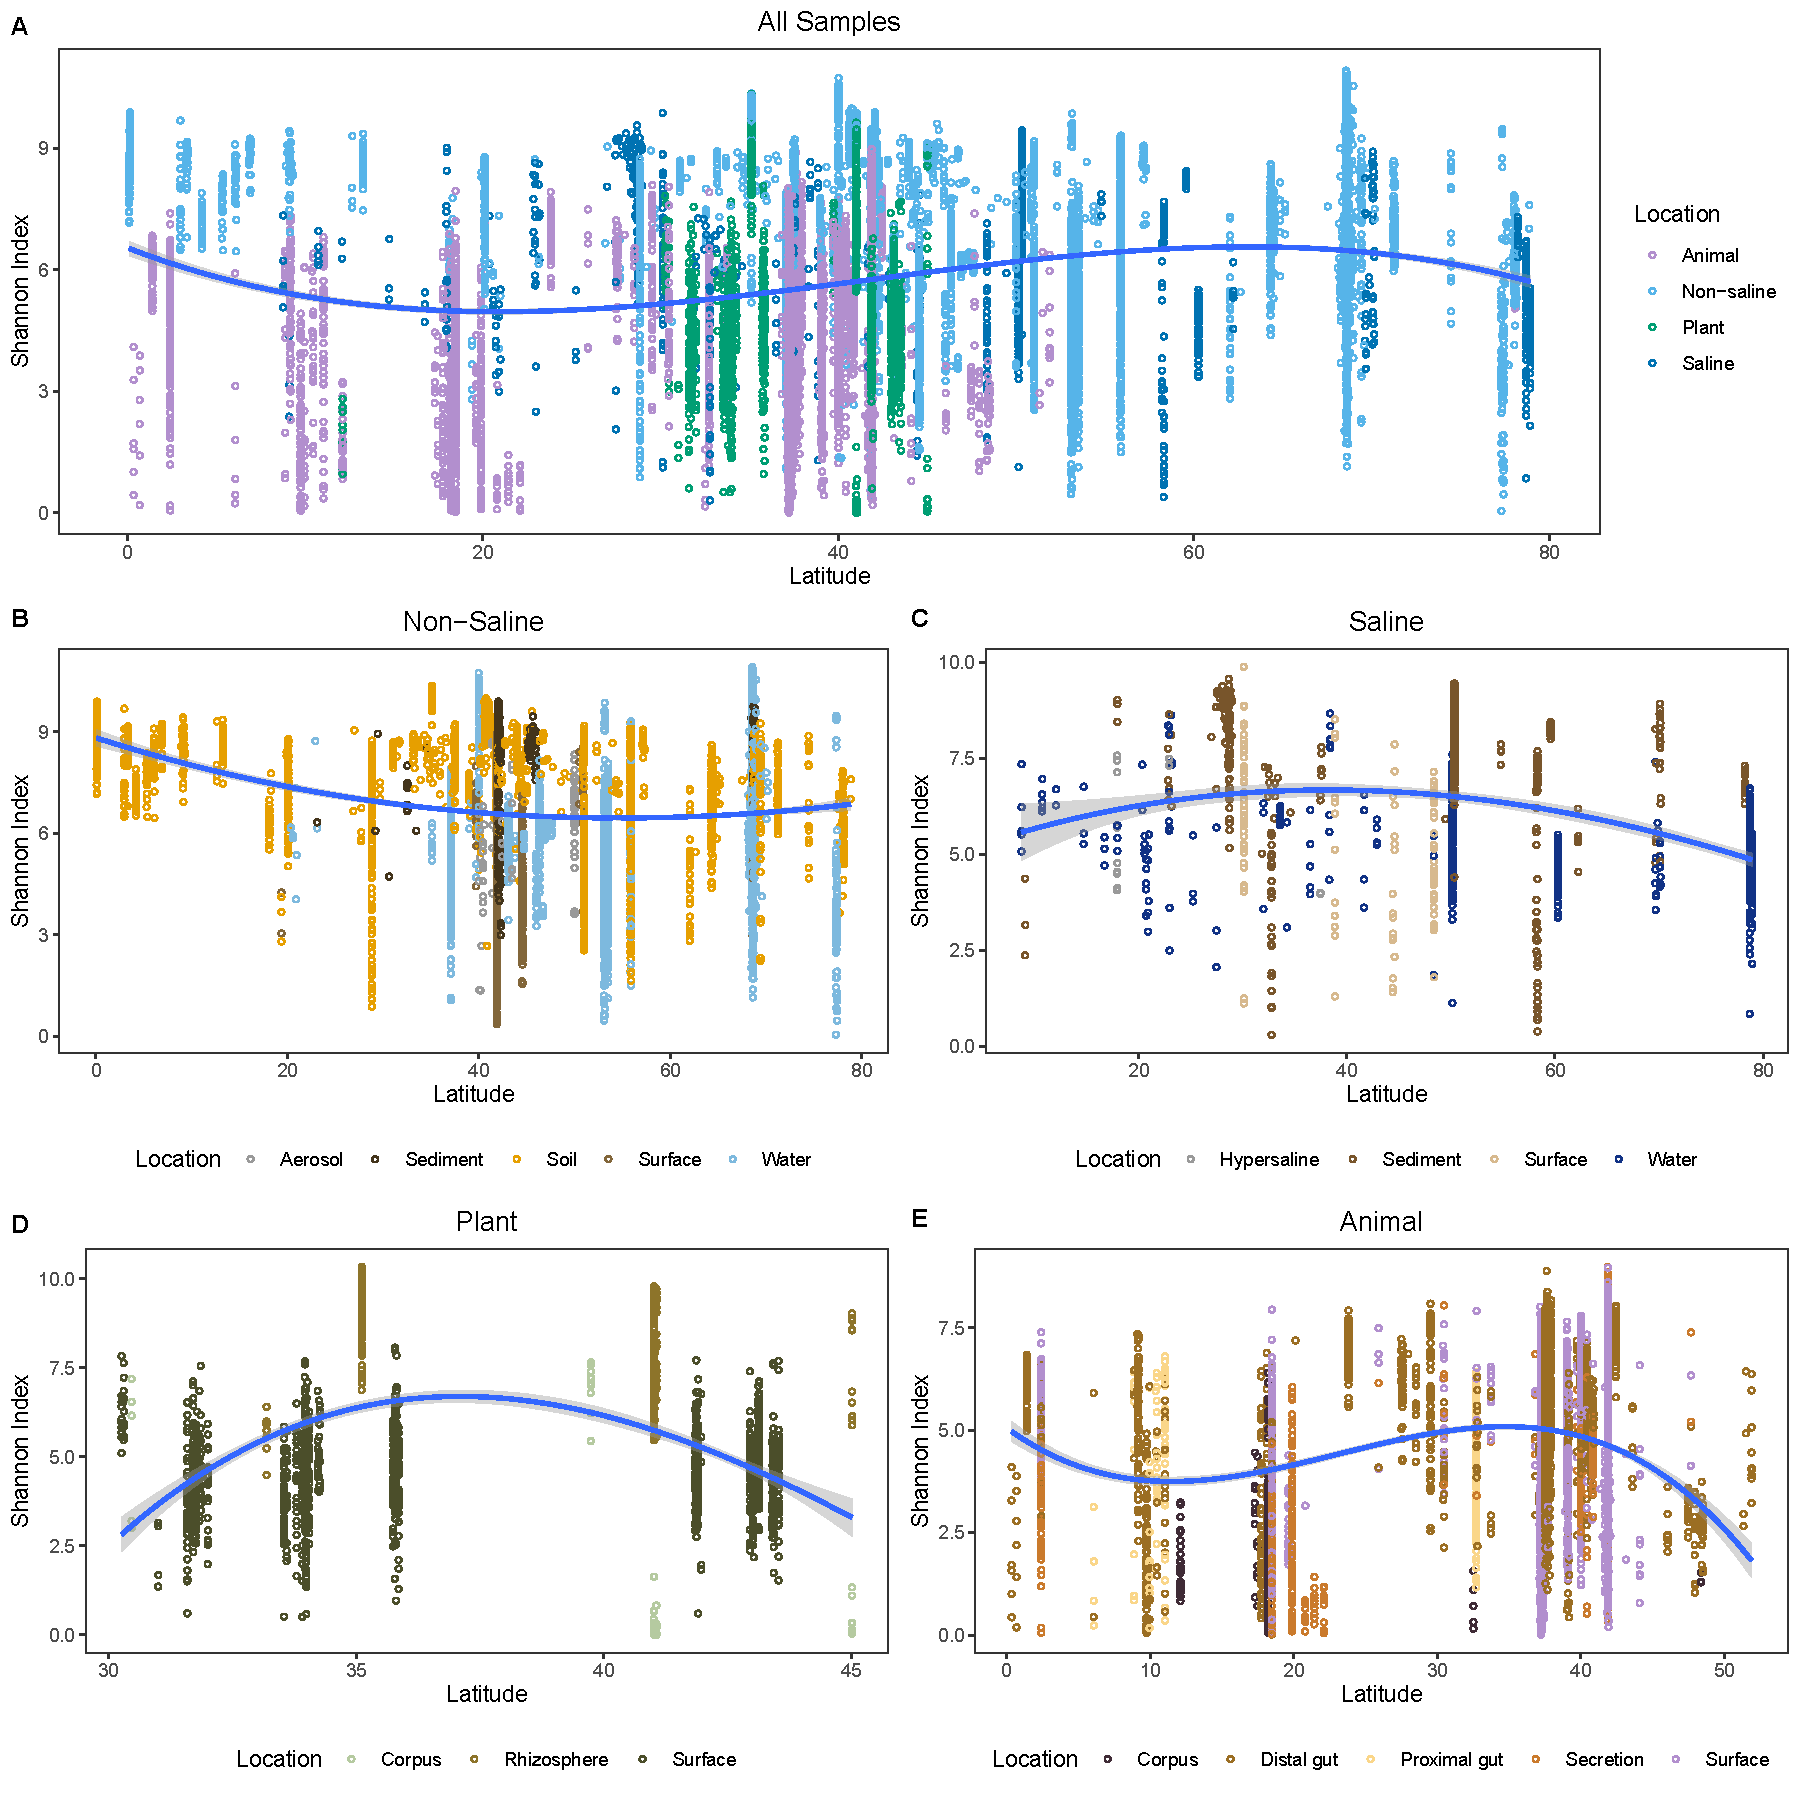
\includegraphics[scale=0.33]{./Figures/Shan_lati_empo2}
    \caption{\textbf{The relationship between Shannon index and latitude.} A: Trend of Shannon index with latitude for samples in the whole dataset. B: Trend of Shannon index with latitude for non-saline samples. C: Trend of Shannon index with latitude for saline samples. D: Trend of Shannon index with latitude for plant samples. E: Trend of Shannon index with latitude for animal samples.}
    \label{fig:Shan_lati}
\end{figure}

\begin{figure}[H]
    \centering
    \includegraphics[scale=0.33]{./Figures/OO_lati_empo3}
    \caption{\textbf{The relationship between observed OTUs and latitude.} A: Trend of observed OTUs with latitude for soil samples. B: Trend of observed OTUs with latitude for non-saline water (water and sediment) samples. C: Trend of observed OTUs with latitude for saline water (water and sediment) samples. D: Trend of observed OTUs with latitude for non-saline sediment samples. E: Trend of observed OTUs with latitude for non-saline surface samples. F: Trend of observed OTUs with latitude for non-saline water samples. G: Trend of observed OTUs with latitude for saline sediment samples. H: Trend of observed OTUs with latitude for saline surface samples. I: Trend of observed OTUs with latitude for saline water samples. J: Trend of observed OTUs with latitude for animal surface samples. K: Trend of observed OTUs with latitude for plant surface samples. L: Trend of observed OTUs with latitude for plant rhizosphere samples.}
    \label{fig:OO_lati3}
\end{figure}


\begin{figure}[H]
    \centering
    \includegraphics[scale=0.33]{./Figures/Shan_lati_empo3}
    \caption{\textbf{The relationship between Shannon index and latitude.} A: Trend of Shannon index with latitude for soil samples. B: Trend of Shannon index with latitude for non-saline water (water and sediment) samples. C: Trend of Shannon index with latitude for saline water (water and sediment) samples. D: Trend of Shannon index with latitude for non-saline sediment samples. E: Trend of Shannon index with latitude for non-saline surface samples. F: Trend of Shannon index with latitude for non-saline water samples. G: Trend of Shannon index with latitude for saline sediment samples. H: Trend of Shannon index with latitude for saline surface samples. I: Trend of Shannon index with latitude for saline water samples. J: Trend of Shannon index with latitude for animal surface samples. K: Trend of Shannon index with latitude for plant surface samples. L: Trend of Shannon index with latitude for plant rhizosphere samples.}
    \label{fig:Shan_lati3}
\end{figure}


\subsection{The relationships between alpha diversity and environmental variables}

\begin{figure}[H]
    \centering
    \includegraphics[scale=0.15]{./Figures/PairsPlot}
    \caption{\textbf{The relationship between alpha diversity indices, temperature, pH and latitude.} A: The relationship between Chao1 index, temperature, pH and latitude. B: The relationship between observed OTUs, temperature, pH and latitude. C: The relationship between Shannon index, temperature, pH and latitude..}
    \label{fig:Pairs}
\end{figure}

\begin{figure}[H]
    \centering
    \includegraphics[scale=0.33]{./Figures/OO_LM_PM_simpleTpL}
    \caption{\textbf{Linear and polynomial regression models of Observed OTUs with a single environmental variable.} A: Linear model of Observed OTUs versus temperature. B: Linear model of Observed OTUs versus pH. C: Linear model of Observed OTUs versus latitude. D: Polynomial regression model of Observed OTUs versus temperature. E: Polynomial regression model of Observed OTUs versus pH. F: Polynomial regression model of Observed OTUs versus latitude.}
    \label{fig:OO_simpleTpL}
\end{figure}

\begin{figure}[H]
    \centering
    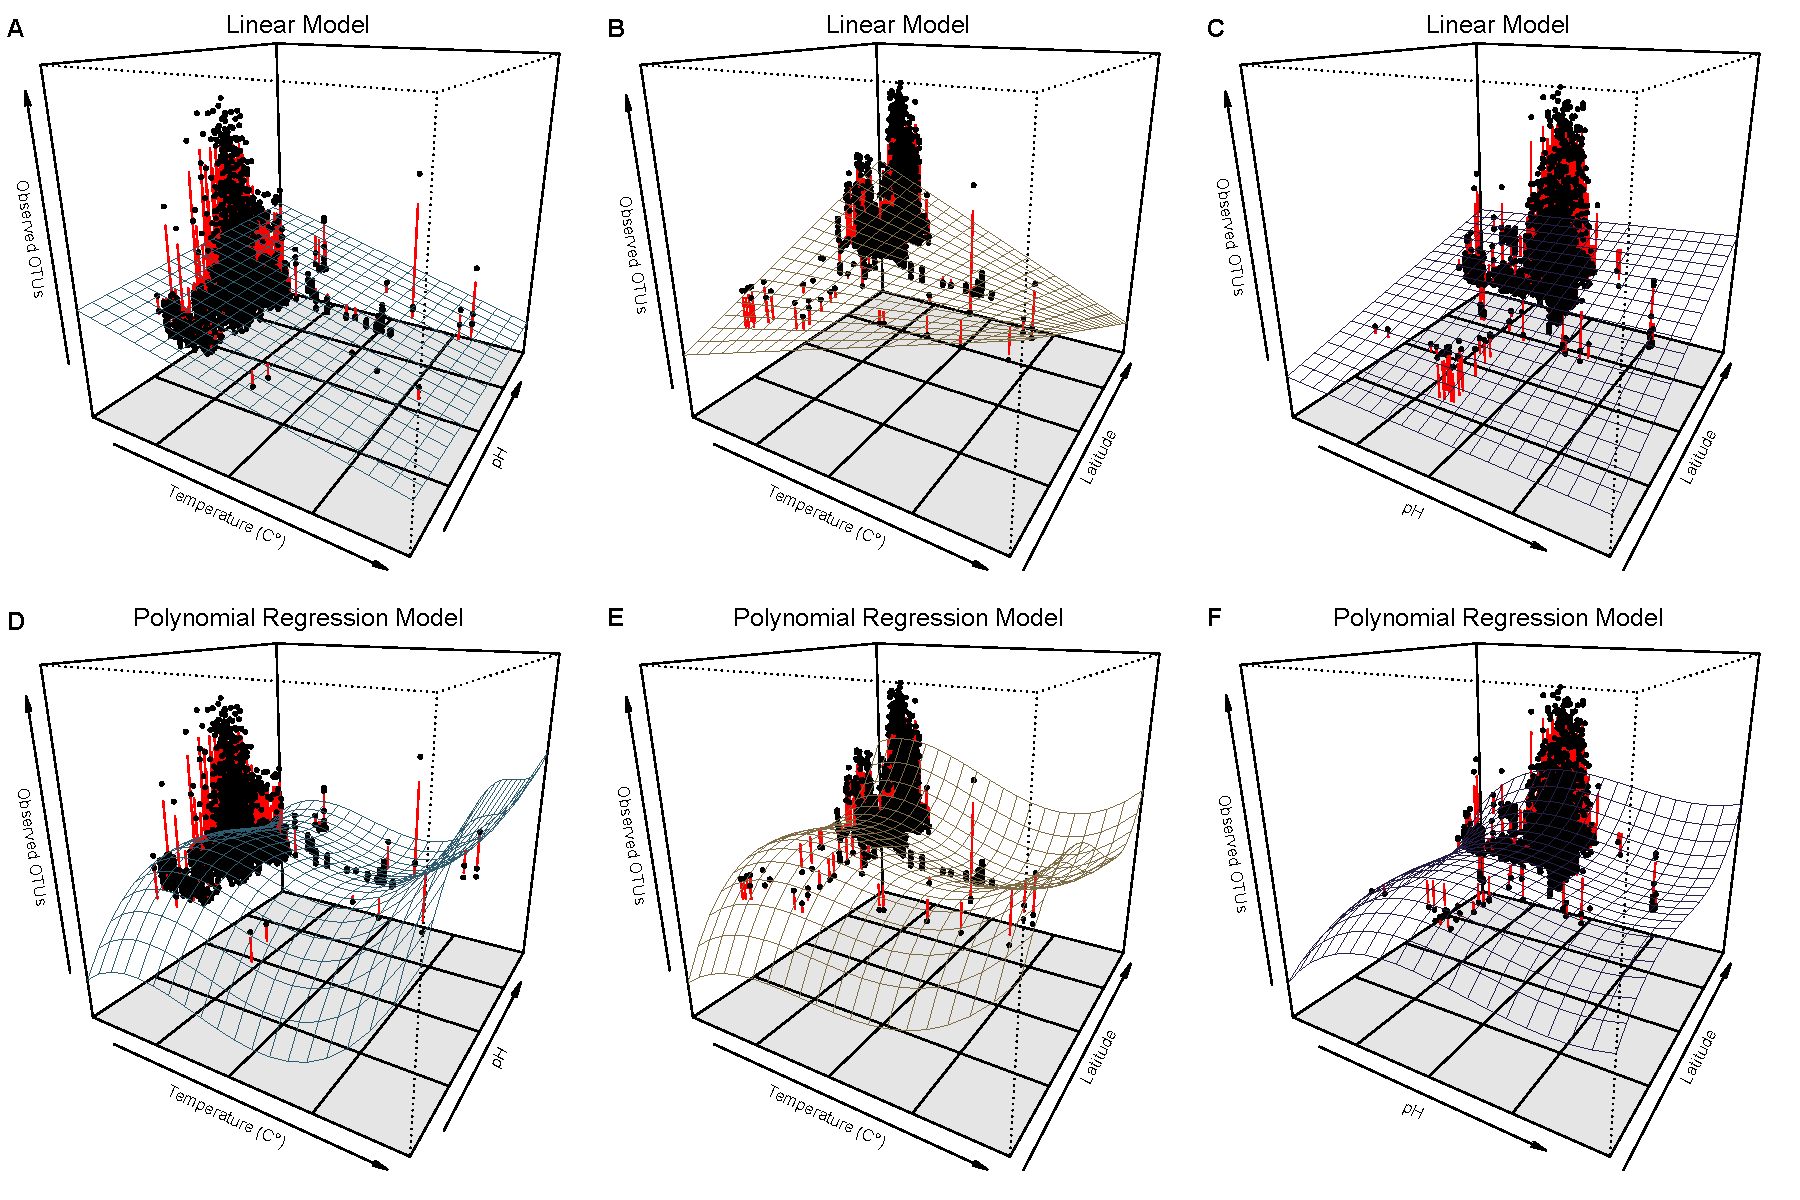
\includegraphics[scale=0.33]{./Figures/OO_LM_PM_all_2EVs_3D}
    \caption{\textbf{Linear and polynomial regression models of Observed OTUs with two environmental variables.} A: Linear model of Observed OTUs versus temperature and pH. B: Linear model of Observed OTUs versus temperature and latitude. C: Linear model of Observed OTUs versus pH and latitude. D: Polynomial regression model of Observed OTUs versus temperature and pH. E: Polynomial regression model of Observed OTUs versus temperature and latitude. F: Polynomial regression model of Observed OTUs versus pH and latitude.}
    \label{fig:OO_2EVs}
\end{figure}

\begin{figure}[H]
    \centering
    \includegraphics[scale=0.33]{./Figures/Shan_LM_PM_simpleTpL}
    \caption{\textbf{Linear and polynomial regression models of Shannon index with a single environmental variable.} A: Linear model of Shannon index versus temperature. B: Linear model of Shannon index versus pH. C: Linear model of Shannon index versus latitude. D: Polynomial regression model of Shannon index versus temperature. E: Polynomial regression model of Shannon index versus pH. F: Polynomial regression model of Shannon index versus latitude.}
    \label{fig:Shan_simpleTpL}
\end{figure}

\begin{figure}[H]
    \centering
    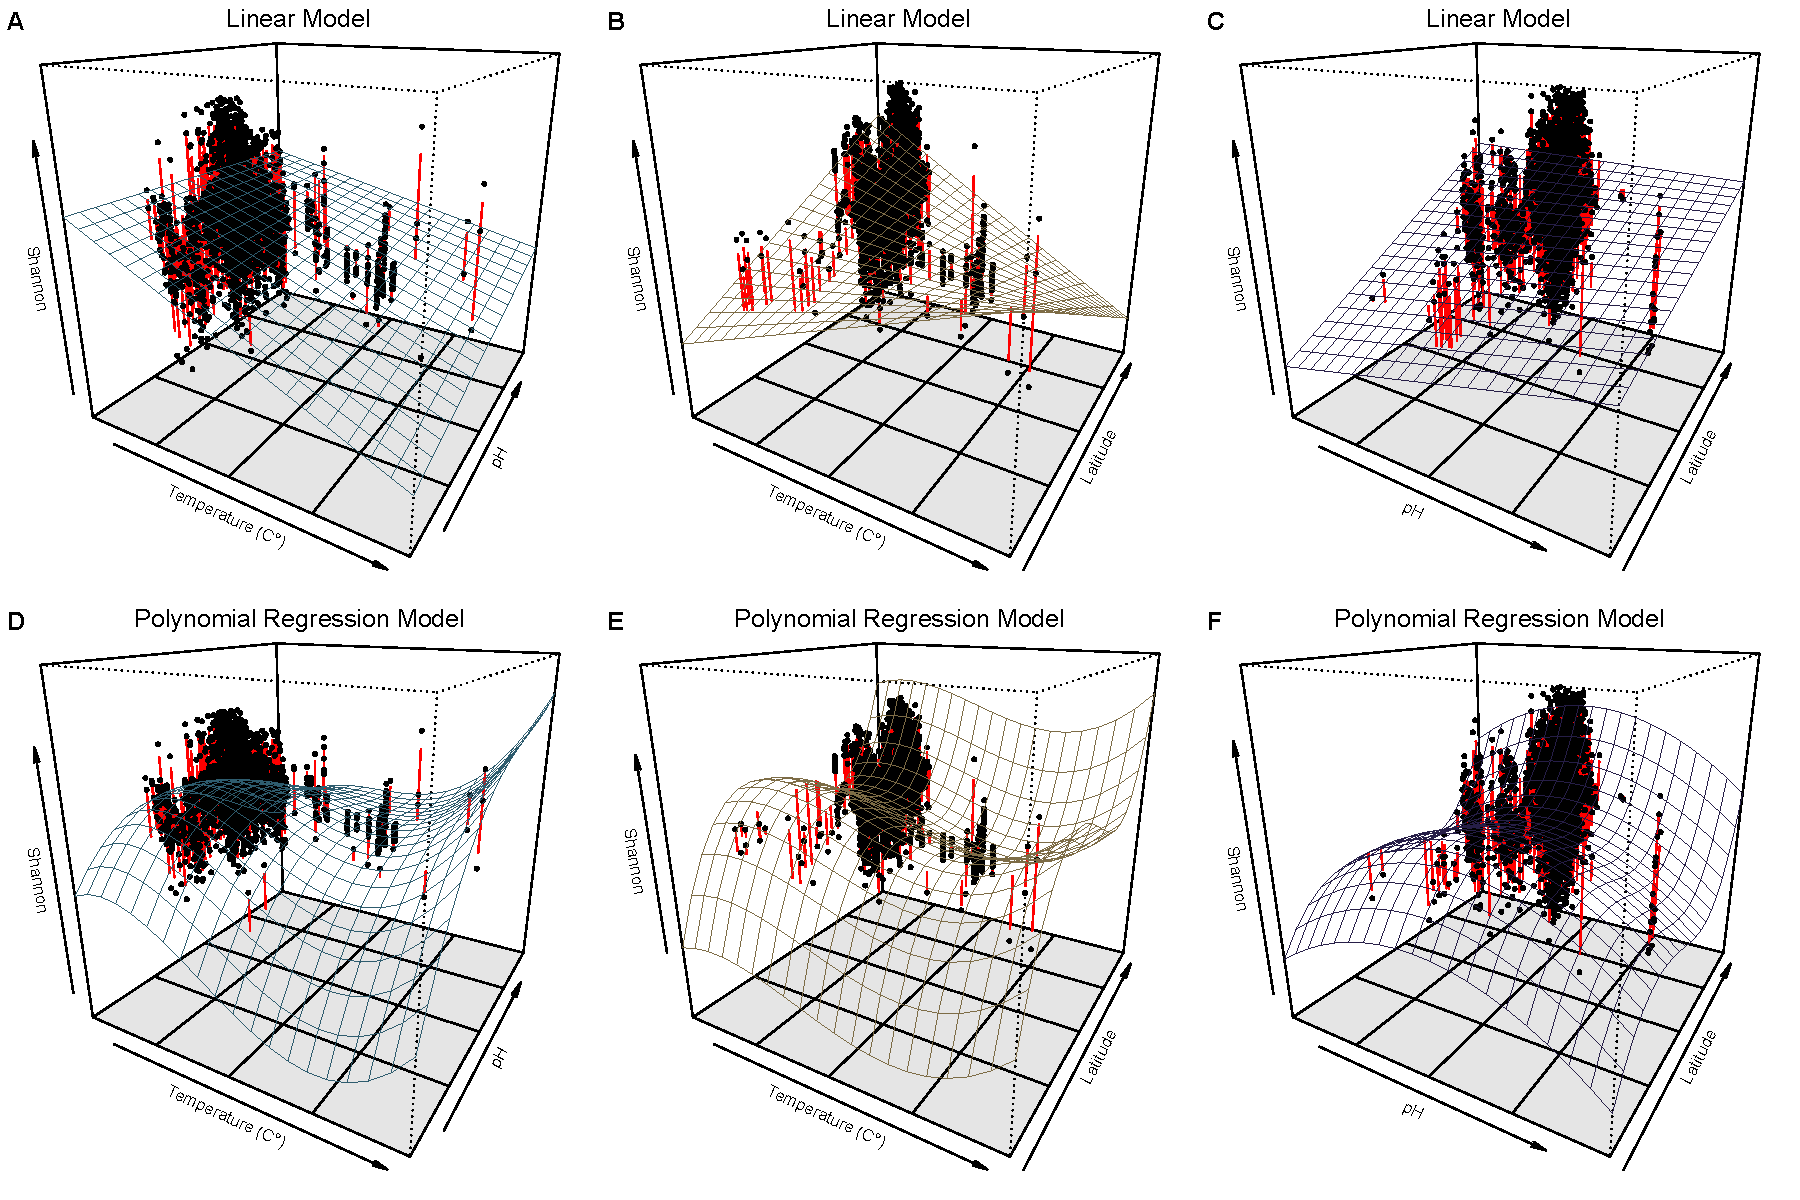
\includegraphics[scale=0.33]{./Figures/Shan_LM_PM_all_2EVs_3D}
    \caption{\textbf{Linear and polynomial regression models of Shannon index with two environmental variables.} A: Linear model of Shannon index versus temperature and pH. B: Linear model of Shannon index versus temperature and latitude. C: Linear model of Shannon index versus pH and latitude. D: Polynomial regression model of Shannon index versus temperature and pH. E: Polynomial regression model of Shannon index versus temperature and latitude. F: Polynomial regression model of Shannon index versus pH and latitude.}
    \label{fig:Shan_2EVs}
\end{figure}

\begin{table}[H]
    \caption{R-square of the EMPO3 models between Chao1 index, observed OTUs and Shannon index and environmental variables.}
    \centering
    \begin{tabular}{ |m{1cm}<{\centering}|m{1.3cm}<{\centering}|m{1.3cm}<{\centering}|m{1.3cm}<{\centering}|m{1.3cm}<{\centering}|m{1.3cm}<{\centering}|m{1.3cm}<{\centering}|m{1.3cm}<{\centering}|m{1.3cm}<{\centering}|m{1.3cm}<{\centering}|} 
    \hline
     $R^{2}$ (NS-Water) & Chao1 (LM) & Chao1 (PM) & Chao1 (RF) & Shannon (LM) & Shannon (PM) & Shannon (RF) & OTUs (LM) & OTUs (PM) & OTUs (RF) \\
     \hline
    T*p*L & 0.1781 & 0.1957 & 0.3979 & 0.2236 & 0.2355 & 0.322 & 0.1665 & 0.1829 & 0.3909 \\
    T*p & NULL & 0.1027 & 0.14 & 0.01416 & 0.1145 & 0.1534 & NULL & 0.09218 & 0.1284 \\
    T*L & 0.1458 & 0.1663 & 0.4269 & 0.2064 & 0.2165 & 0.3233 & 0.1363 & 0.1544 & 0.4304 \\
    p*L & NULL & 0.1344 & 0.4308 & 0.1962 & 0.2064 & 0.3186 & NULL & 0.1233 & 0.4149 \\
    T & 0.003247 & 0.06321 & 0.0186 & 0.0103 & 0.0522 & NULL & 0.004906 & 0.05587 & 0.0116 \\
    p & NULL & 0.06568 & 0.0994 & 0.003669 & 0.09646 & 0.1128 & NULL & 0.06064 & 0.0837 \\
    L & 0.1295 & 0.1327 & 0.4653 & 0.1854 & 0.1961 & 0.3463 & 0.116 & 0.1206 & 0.4609 \\
    \hline
    \hline
     $R^{2}$ (NS-Surf) & Chao1 (LM) & Chao1 (PM) & Chao1 (RF) & Shannon (LM) & Shannon (PM) & Shannon (RF) & OTUs (LM) & OTUs (PM) & OTUs (RF) \\
     \hline
    T*p*L & 0.6096 & 0.6594 & 0.6567 & 0.4957 & 0.5505 & 0.4803 & 0.5749 & 0.6241 & 0.6213 \\
    T*p & 0.4078 & 0.4895 & 0.6621 & 0.273 & 0.2916 & 0.4764 & 0.3603 & 0.4297 & 0.6243 \\
    T*L & NULL & 0.6011 & 0.6373 & NULL & 0.4443 & 0.463 & NULL & 0.5543 & 0.5965 \\
    p*L & 0.2897 & 0.558 & 0.642 & 0.1716 & 0.393 & 0.4681 & 0.2448 & 0.5036 & 0.6008 \\
    T & 0.2403 & 0.4724 & 0.6525 & 0.1373 & 0.2693 & 0.4696 & 0.205 & 0.4216 & 0.6164 \\
    p & 0.038 & 0.3264 & 0.6354 & 0.03825 & 0.1939 & 0.4225 & 0.03848 & 0.276 & 0.5914 \\
    L & NULL & 0.285 & 0.2741 & NULL & 0.2714 & 0.2542 & NULL & 0.2773 & 0.2656 \\
    \hline
    \hline
     $R^{2}$ (S-Sedi) & Chao1 (LM) & Chao1 (PM) & Chao1 (RF) & Shannon (LM) & Shannon (PM) & Shannon (RF) & OTUs (LM) & OTUs (PM) & OTUs (RF) \\
     \hline
    T*p*L & 0.5044 & 0.5044 & 0.4741 & NULL & NULL & 0.4035 & 0.578 & 0.578 & 0.5295 \\
    T*p & NULL & 0.4832 & 0.4342 & NULL & NULL & 0.3925 & NULL & 0.5499 & 0.5121 \\
    T*L & NULL & 0.4758 & 0.4672 & NULL & NULL & 0.3988 & NULL & 0.5554 & 0.5355 \\
    p*L & 0.5016 & 0.5018 & 0.4709 & 0.4109 & NULL & 0.3988 & 0.5717 & 0.5795 & 0.5416 \\
    T & 0.01735 & 0.4322 & 0.4677 & NULL & 0.1402 & 0.3899 & 0.01459 & 0.5115 & 0.5303 \\
    p & NULL & 0.09837 & 0.4275 & NULL & 0.1067 & 0.3854 & NULL & 0.1161 & 0.4941 \\
    L & 0.449 & 0.4559 & 0.447 & 0.3903 & 0.4102 & 0.4007 & 0.5302 & 0.545 & 0.5301 \\
    \hline
    \end{tabular}    
    \label{tab:EMPO3models}
\end{table}

\begin{table}[H]
    \caption{R-square of the local samples models between Chao1 index, observed OTUs and Shannon index and environmental variables. Local 1, 2 and 3 are Yellowstone National Park, Großer Stechlinsee and Toolik Lake respectively.}
    \centering
    \begin{tabular}{ |m{1.3cm}<{\centering}|m{1.2cm}<{\centering}|m{1.2cm}<{\centering}|m{1.2cm}<{\centering}|m{1.4cm}<{\centering}|m{1.4cm}<{\centering}|m{1.4cm}<{\centering}|m{1.3cm}<{\centering}|m{1.3cm}<{\centering}|m{1.2cm}<{\centering}|} 
    \hline
     $R^{2}$ & Chao1 (LM) & Chao1 (PM) & Chao1 (RF) & Shannon (LM) & Shannon (PM) & Shannon (RF) & OTUs (LM) & OTUs (PM) & OTUs (RF) \\
     \hline
    Local 1 T*p & 0.4719 & 0.4918 & 0.6588 & 0.2912 & 0.3152 & 0.4806 & 0.412 & 0.433 & 0.6205 \\
    Local 2 T*p & NULL & NULL & NULL & 0.04069 & 0.04874 & NULL & 0.009332 & 0.0143 & NULL \\
    Local 3 T*p & 0.05701 & 0.08249 & 0.0461 & 0.04255 & 0.05284 & 0.0098 & 0.0594 & 0.08191 & 0.0555 \\
    Local 1 T & 0.2438 & 0.473 & 0.6529 & 0.1433 & 0.267 & 0.4715 & 0.2093 & 0.04204 & 0.6159 \\
    Local 2 T & NULL & 0.003542 & NULL & 0.009679 & 0.009679 & NULL & 0.001895 & 0.003983 & NULL \\
    Local 3 T & 0.01907 & 0.06512 & 0.0185 & 0.03076 & 0.04849 & NULL & 0.0247 & 0.0647 & 0.0272 \\
    Local 1 p & 0.2981 & 0.4996 & 0.6343 & 0.1678 & 0.289 & 0.4266 & 0.2529 & 0.4368 & 0.5872 \\
    Local 2 p & NULL & NULL & NULL & 0.03141 & 0.03629 & NULL & 0.007482 & 0.01022 & NULL \\
    Local 3 p & NULL & 0.00248 & NULL & NULL & NULL & NULL & NULL & 0.001819 & NULL \\
    \hline
    \end{tabular}    
    \label{tab:localmodels}
\end{table}

\end{document}

\end{spacing}
\end{document}